%% Based on a TeXnicCenter-Template by Gyorgy SZEIDL.
%%%%%%%%%%%%%%%%%%%%%%%%%%%%%%%%%%%%%%%%%%%%%%%%%%%%%%%%%%%%%

%----------------------------------------------------------
%
\documentclass{report}%
%
%----------------------------------------------------------
% This is a sample document for the standard LaTeX Report Class
% Class options
%       --  Body text point size:
%                        10pt (default), 11pt, 12pt
%       --  Paper size:  letterpaper (8.5x11 inch, default)
%                        a4paper, a5paper, b5paper,
%                       legalpaper, executivepaper
%       --  Orientation (portrait is the default):
%                       landscape
%       --  Printside:  oneside (default), twoside
%       --  Quality:    final (default), draft
%       --  Title page: titlepage, notitlepage
%       --  Columns:    onecolumn (default), twocolumn
%       --  Start chapter on left:
%                       openright(no), openany (default)
%       --  Equation numbering (equation numbers on right is the default)
%                       leqno
%       --  Displayed equations (centered is the default)
%                       fleqn (flush left)
%       --  Open bibliography style (closed bibliography is the default)
%                       openbib
% For instance the command
%          \documentclass[a4paper,12p,leqno]{report}
% ensures that the paper size is a4, fonts are typeset at the size 12p
% and the equation numbers are on the left side.
%
\usepackage{amsmath}%
\usepackage{amsfonts}%
\usepackage{amssymb}%
\usepackage{graphicx}
%----------------------------------------------------------
\usepackage{url}
\usepackage{tabularx}
%\usepackage{tablefootnote}
\usepackage[square,sort,comma,numbers]{natbib}
\usepackage{chapterbib}
\usepackage{hyperref}
\usepackage{url}
\usepackage{doi}
\usepackage{listings}
\usepackage{color}
%----------------------------------------------------------
% Define colors:
\definecolor{dkgreen}{rgb}{0,0.6,0}
\definecolor{gray}{rgb}{0.5,0.5,0.5}
\definecolor{mauve}{rgb}{0.58,0,0.82}
% Define language
\lstdefinelanguage{torxakis}
{
  % list of keywords
  morekeywords={
    PROCDEF,
    FUNCDEF
  },
  sensitive=false, % keywords are not case-sensitive
  morecomment=[l]{//}, % l is for line comment
  morecomment=[s]{/*}{*/}, % s is for start and end delimiter
  morestring=[b]" % defines that strings are enclosed in double quotes
}
% Define environment:
\lstset{frame=tb,
  language=torxakis,
  aboveskip=3mm,
  belowskip=3mm,
  showstringspaces=false,
  columns=flexible,
  basicstyle={\small\ttfamily},
  numbers=none,
  numberstyle=\tiny\color{gray},
  keywordstyle=\color{blue},
  commentstyle=\color{dkgreen},
  stringstyle=\color{mauve},
  breaklines=true,
  breakatwhitespace=true,
  tabsize=3
}
%----------------------------------------------------------
\newcommand{\txs}{TorXakis}
\newcommand{\mcrl}{mCRL2}
\newcommand{\inlinecode}[1]{{\lstinline[language=torxakis]{#1}}}
\newcommand{\istep}{\texttt{ISTEP}}
\newcommand{\cistep}{\texttt{CISTEP}}
\newcommand{\true}{\textbf{true}}
\newcommand{\false}{\textbf{false}}
\newcommand{\shPair}[2]{\langle\;#1,\;#2\;\rangle}
\newcommand{\labeledas}[1]{labeled as `#1'}
\newcommand{\labeledaseither}[2]{labeled as `#1' or `#2'}
\newcommand{\removelabelfrom}[1]{remove the label `#1' from}
\newcommand{\varsof}[1]{\text{vars}(#1)}
\newcommand{\sortof}[1]{\text{sort}(#1)}
\newcommand{\flsortof}[1]{\text{fl}(\sortof{#1})}
%----------------------------------------------------------
\setlength\parindent{0pt}
%----------------------------------------------------------
%\makeatletter
%\newcommand\footnoteref[1]{\protected@xdef\@thefnmark{\ref*{#1}}\@footnotemark}
%\makeatother
%----------------------------------------------------------
\newtheorem{theorem}{Theorem}
\newtheorem{acknowledgement}[theorem]{Acknowledgement}
\newtheorem{algorithm}[theorem]{Algorithm}
\newtheorem{axiom}[theorem]{Axiom}
\newtheorem{case}[theorem]{Case}
\newtheorem{claim}[theorem]{Claim}
\newtheorem{conclusion}[theorem]{Conclusion}
\newtheorem{condition}[theorem]{Condition}
\newtheorem{conjecture}[theorem]{Conjecture}
\newtheorem{corollary}[theorem]{Corollary}
\newtheorem{criterion}[theorem]{Criterion}
\newtheorem{definition}[theorem]{Definition}
\newtheorem{example}[theorem]{Example}
\newtheorem{exercise}[theorem]{Exercise}
\newtheorem{lemma}[theorem]{Lemma}
\newtheorem{notation}[theorem]{Notation}
\newtheorem{problem}[theorem]{Problem}
\newtheorem{proposition}[theorem]{Proposition}
\newtheorem{remark}[theorem]{Remark}
\newtheorem{solution}[theorem]{Solution}
\newtheorem{summary}[theorem]{Summary}
\newenvironment{proof}[1][Proof]{\textbf{#1.} }{\ \rule{0.5em}{0.5em}}
%----------------------------------------------------------
\begin{document}

\title{LPE operations}
\author{Djurre van der Wal}
\date{\today}
\maketitle
\tableofcontents

\chapter{Getting started}

\section{Introduction}

\txs{} offers several techniques to symbolically manipulate \txs{} models.
This section gives an overview of how to get started with these techniques.

\section{Installation}

\begin{enumerate}
\item Download \texttt{stack} as described on
\begin{align*}
\texttt{https://docs.haskellstack.org/en/stable/README/}
\end{align*}

and install it.

\item Download and install an SMT solver such as
\begin{align*}
\texttt{Z3 version 4.8.3 - 64 bit - build hashcode cf4bf7b591b6}
\end{align*}

Add the binaries of the SMT solver to \texttt{PATH}.
\item Clone the \texttt{develop} branch from
\begin{align*}
\texttt{https://github.com/ikbendedjurre/txs-develop}
\end{align*}
\item In a terminal, navigate to the repository directory and run
\begin{itemize}
\item \texttt{stack -v setup}
\item \texttt{stack -v --profile build}
\end{itemize}
\item The \txs{} binaries can be found in
\begin{align*}
\texttt{/.stack-work/install/23f9efff/bin}
\end{align*}

in the repository directory (the \texttt{23f9efff} hash is build-dependent).

Add the binaries to \texttt{PATH} (there may be a way to do this more easily with \texttt{stack}).
\end{enumerate}

\section{Starting \txs{}} \label{starttxs}

\begin{enumerate}
\item Make it so that \texttt{txsserver.exe} and \texttt{torxakis.exe} are in \texttt{PATH}.
\item Start two terminals, one for the \txs{} server and one for the \txs{} client -- this has the advantage that errors that occur on the server-side will be visible.
\item In both terminals, navigate to the directory with a \txs{} specification file (such as \texttt{example.txs}).
\item In one terminal, run \texttt{txsserver --no-smt-log 50001} where the number \texttt{50001} is the port number that the \txs{} server will listen for clients.
\item In the other terminal, run \texttt{torxakis 50001 example.txs}.
\end{enumerate}

\section{Process linearization} \label{processlinearization}

The symbolic manipulation of \txs{} models requires the processes that underlie those models to be in \emph{LPE form} (see \ref{lpeform}).
To make a \txs{} process linear in practice, do the following:

\begin{enumerate}
\item Start \txs{} (see \ref{starttxs}).
\item Run
\begin{align*}
\texttt{lpe Model}
\end{align*}

in the client terminal, where \texttt{Model} is the name of the model in the \txs{} specification file.
\txs{} will attempt to linearize the processes that underlie that model.

Note that not all \txs{} models are linearizable.
For those models, the \texttt{lpe} command will fail, with an error reported in the server terminal.
\item If successful, the \texttt{lpe} command prints the name of a new \txs{} model that was created.
This model can be manipulated symbolically (see \ref{modelmanipulation}).
\end{enumerate}

\section{Model manipulation} \label{modelmanipulation}

After \ref{starttxs} and \ref{processlinearization}, symbolic manipulation of a \txs{} model can begin.
To do this, use the \texttt{lpeop} command in the client terminal.

The \texttt{lpeop} command has 3 space-separated arguments. In order, these arguments are:

\begin{itemize}
\item A chain of LPE operations.
LPE operations are represented by their name, such as \texttt{cstelm} or \texttt{loop} (see \ref{lpeoperations}).
These names are separated by the symbol \texttt{->}.

LPE operations in the chain are executed from left to right, passing their output to the next LPE operation as input.
If a problem occurs, the process ends immediately.
Otherwise, the final output model is saved as a new model.
\item The name of the input model.
The process that underlies the input model should be in LPE form (see \ref{lpeform}).
\item A base name \textit{base} for generated output.
The name is primarily used for the output model (if any), the underlying process of which is in LPE form.
However, LPE operations may adopt the name for their own purposes.
The \texttt{export} operation, for example, will create a file by that name with the \texttt{.txs} extension.

It is possible to use the \texttt{\%i} token in the base name.
This will insert the current counter value into the name.
Use the \texttt{inc} command to increase the counter (which starts at 1).
\end{itemize}

\section{Unit tests}

\begin{enumerate}
\item In a terminal, navigate to the repository directory.
\item Execute \texttt{stack -v --profile test lpeops}.
\end{enumerate}

\section{Benchmarks}

\subsection{Generation (Windows OS only)}
First, benchmark files must be generated.
This is done via script.

\begin{enumerate}
\item Navigate to \texttt{/examps} and open the file
\begin{align*}
\texttt{generateBenchmarkData.bat}
\end{align*}

\item Change \texttt{TXSDIR} to the directory where the \txs{} source files are located.
Among others, it should contain the following sub-directories:
\begin{center}
\texttt{examps} \\
\texttt{sys} \\
\texttt{test}
\end{center}

\item In order to perform different benchmark measurements, change the contents of the function \texttt{:WriteCommands} (line 104, in particular, describes how the model should be produced that is compared to the original model and the linearized model).

\item Run \texttt{generateBenchmarkData.bat} and wait for it to finish.
\end{enumerate}

\subsection{Execution}
The main benchmark file of \txs{},
\begin{align*}
\texttt{/test/sqatt/src/Benchmarks/All.txs}
\end{align*}

has been changed, and so the benchmark for LPE operations is started in the same way as the original benchmark:

\begin{enumerate}
\item In a terminal, navigate to \texttt{/test/sqatt} in the repository directory.
\item Execute
\begin{center}
\texttt{stack -v --profile bench --ba} \\
\texttt{"--output data.html --csv data.csv --time-limit 1"}
\end{center}

The benchmark spends a maximum of 1 second on each part of the benchmark (default is 5 seconds).
If there are no failures, the benchmark results will be exported to \texttt{data.html} and \texttt{data.csv} (note that previous results are not deleted from \texttt{data.csv}).
For more benchmark parameters, see \url{http://www.serpentine.com/criterion/tutorial.html}.

\item Wait for the benchmark to finish.
\end{enumerate}






\chapter{LPE operations} \label{lpeoperations}

\section{Introduction}

Techniques that symbolically manipulate \txs{} models are applied via \emph{LPE operations}.
LPE operations are divided into 3 categories:

\begin{itemize}
\item Basic operations, which make it possible for the user to chain LPE operations together in a convenient manner;
\item Analysis operations, which give information about their input LPE; and
\item Rewrite operations, which may significantly change the input LPE.
\end{itemize}

\section{Basic operations}

Table~\ref{basiclpeops:table} gives an overview of the basic LPE operations.

\begin{table}[!ht]
\begin{center}
\begin{tabularx}{\linewidth}{l|X|}
\textbf{Operation} & \textbf{Description} \\ \hline
\texttt{stop} & End the chain of operations immediately. \\ \hline
\texttt{valid} & Validate the input LPE. \\ \hline
\texttt{show} & Print the input LPE to the terminal. \\ \hline
\texttt{show*} & Same as \texttt{show}, but the output is compilable \txs{} code, and identifiers in the output have been shortened for readability. \\ \hline
\texttt{export} & Save the input LPE to \textit{base}\texttt{.txt}. \\ \hline
\texttt{export*} & Same as \texttt{export}, but the output is compilable \txs{} code, and identifiers in the output have been shortened for readability. \\ \hline
\texttt{loop} & If the input LPE has not been encountered before, restart from the most recent \texttt{start} command, or from the first operation if no \texttt{start} command has been encountered yet. \\ \hline
\texttt{loop*}$N$ & Same as \texttt{loop}, but the number of restarts is limited to $N$. \\ \hline
\texttt{start} & Set the location where the command chain should continue when looping. \\ \hline
\texttt{inc} & Increase the counter that can be used in \textit{base}. \\ \hline
\end{tabularx}
\caption{Basic LPE operations.}
\label{basiclpeops:table}
\end{center}
\end{table}

\section{Analysis operations}

Table~\ref{lpeanalysisops:table} gives an overview of the LPE analysis operations.

\begin{table}[!ht]
\begin{center}
\begin{tabularx}{\linewidth}{l|X|}
\textbf{Operation} & \textbf{Description} \\ \hline
\texttt{isdet} & Return the input LPE after assessing whether it is deterministic. May yield false negatives. \\ \hline
\texttt{mcrl2} & Convert the current LPE to an \mcrl{} specification (so that \mcrl{} can analyze it), and save it to \textit{base}\texttt{.mcrl2}. \\ \hline
\texttt{confcheck} & Perform a confluence analysis on the input LPE, and return the input LPE in which confluent \texttt{ISTEP}s have been renamed to \texttt{CISTEP}s. \\ \hline
\texttt{step*}$N$ & Follow a trace of up to $N$ steps through the input LPE. \\ \hline
\end{tabularx}
\caption{LPE analysis operations.}
\label{lpeanalysisops:table}
\end{center}
\end{table}

\section{Rewrite operations}

Table~\ref{lperewriteops:table} gives an overview of the LPE rewrite operations.
Table~\ref{lperewriteopsprops:table} shows the equivalence that is preserved by each rewrite operation:
\begin{itemize}
\item \textbf{u-ioco}: Underspecified input-output conformance.
\item \textbf{br. bis.}: Branching bisimulation.
\item \textbf{strong bis.}: Strong bisimulation.
\item \textbf{state sp. equiv.}: State space equivalence.
\end{itemize}

\begin{table}[!ht]
\begin{center}
\begin{tabularx}{\linewidth}{l|X|}
\textbf{Operation} & \textbf{Description} \\ \hline
\texttt{clean} & Remove summands of which it can be established that its behavior is also part of another summand in the same LPE; and remove summands of which it can be established via symbolic reachability that they cannot be reached from the initial state. \\ \hline
\texttt{cstelm} & Remove parameters of which it can be established that their value never changes. \\ \hline
\texttt{parelm} & Remove parameters of which it can be established that their value never affects the behavior of the LPE. \\ \hline
\texttt{parreset} & Set parameters of which it can be established via symbolic reachability that their value is no longer used after a specific summand to a default value in the process instantiation of that summand. \\ \hline
\texttt{datareset} & Set parameters of which it can be established via control-flow analysis that their value is no longer used after a specific summand to a default value in the process instantiation of that summand. \\ \hline
\texttt{confelm} & Rewrite the input LPE so that confluent \texttt{ISTEP} summands are prioritized. \\ \hline
\texttt{det} & \textit{Experimental.} Rewrite the input LPE in an attempt to reduce non-determinism. By design, \texttt{det} does not generally remove all non-determinism in one execution because it may not terminate (see if there is a fixed point with \texttt{loop}). \\ \hline
\texttt{uguard} & \textit{Experimental.} Search for underspecified summands and remove them. \\ \hline
\end{tabularx}
\caption{LPE rewrite operations.}
\label{lperewriteops:table}
\end{center}
\end{table}

\begin{table}[!ht]
\begin{center}
\begin{tabularx}{\linewidth}{X|c|c|c|c|}
\textbf{Operation} & \textbf{u-ioco} & \textbf{br. bis.} & \textbf{strong bis.} & \textbf{state sp. equiv.} \\ \hline
\texttt{clean} & Yes & Yes & Yes & Yes \\ \hline
\texttt{cstelm} & Yes & Yes & Yes & Yes$^{*}$ \\ \hline
\texttt{parelm} & Yes & Yes & Yes & No \\ \hline
\texttt{parreset} & Yes & Yes & Yes & No \\ \hline
\texttt{datareset} & Yes & Yes & Yes & No \\ \hline
\texttt{confelm} & Yes & Yes & No & No \\ \hline
\texttt{det} & Yes & Yes & Yes & No \\ \hline
\texttt{uguard} & Yes & No & No & No \\ \hline
\end{tabularx}
\caption{LPE rewrite operations.}
\begin{small}
$^{*}$ State vectors may be smaller; transitions and number of states do not change.
\end{small}
\label{lperewriteopsprops:table}
\end{center}
\end{table}




\chapter{LPE structure}

\section{Introduction}
The LPE operations that are described in this document (see \ref{lpeoperations}) require a \txs{} model as input of which the process is in \emph{linear process equation} (LPE) \emph{form}.
Many, but not all \txs{} processes can be transformed to LPE form using the \texttt{lpe} command of \txs{}.

\section{LPE form} \label{lpeform}

A \txs{} process
\begin{align*}
\texttt{ProcDef} \; [C_1 :: K_1, \cdots{}, C_n :: K_n] \; [p_1 :: T_1, \cdots{}, p_k :: T_k] \; b_\textit{LPE}
\end{align*}

that is identified by $P$ is said to be a in \emph{LPE form} if $b_\textit{LPE}$ follows the grammar of $\textit{LPEBody}$ below:
\begin{align*}
\textit{LPEBody} &::= \texttt{Choice} \; [ \;\! \textit{ActionSmd}, \cdots{}, \textit{ActionSmd} \; ] \\
\textit{ActionSmd} &::= \texttt{ActionPref} \; \textit{ActOffer} \; \textit{ProcInst} \\
\textit{ActOffer} &::= \texttt{ActOffer} \; \textit{ChanOffers} \;\; [ \; h_1, \cdots{}, h_z \; ] \; \textit{VExpr} \\
\textit{ChanOffers} &::= [ \;\! \textit{ChanOffer}, \cdots{}, \textit{ChanOffer} \; ] \\
\textit{ChanOffer} &::= \textit{ChanId} \;\; [\texttt{Quest} \; x_1, \cdots{}, \texttt{Quest} \; x_m] \\
\textit{ChanId} &::= C_1 \;| \cdots{} |\; C_n \;|\; \texttt{ISTEP} \;|\; \texttt{CISTEP} \\
\textit{ProcInst} &::= \texttt{ProcInst} \; P \; \; [ \; C_1, \cdots{}, C_n \; ] \; [\;\!\textit{VExpr}, \cdots{}, \textit{VExpr} \; ]
\end{align*}

Note that
\begin{itemize}
\item $b_\textit{LPE}$ should comply with traditional \txs{} requirements.
More precisely, the communication variables $\{ x_1, \cdots{}, x_m \}$ must match the signature of the \textit{ChanId} channel that occurs in the same rule; and the number of \textit{VExpr}s in the \textit{ProcInst} rule must be equal to $k$ and their sorts must match $[T_1, \cdots{}, T_k]$.
\item it must be the case that the channels that are used in an \textit{ActionSmd} are either all input channels or all output channels.
\item per \textit{ActionSmd}, it must be the case that
\begin{align*}
|\; \{ h_1, \cdots{}, h_z \} \cup \{ x_1, \cdots{}, x_m \} \; | &= z + m \\
(\{ h_1, \cdots{}, h_z \} \cup \{ x_1, \cdots{}, x_m \}) \cap \{ p_1, \cdots{}, p_k \} &= \emptyset{}
\end{align*}
\end{itemize}

\section{Restricted LPE form} \label{restrictedlpeform}

In actuality, it is convenient that processes have a form that is even more restrictive than the LPE form discussed in \ref{lpeform}.
Fortunately, a process that is in LPE form can be converted to restricted LPE form in a way that is reversible.

The restricted LPE form is the same as the regular LPE form, except for the \textit{ActOffer} and \textit{ChanOffers} rules, which have changed to
\begin{align*}
\textit{ActOffer} &::= \texttt{ActOffer} \; \textit{ChanOffers} \;\; [\;] \; \textit{VExpr} \\
\textit{ChanOffers} &::= [ \;\! \textit{ChanOffer} \; ]
\end{align*}

In short, hidden variables are no longer permitted in the restricted LPE form, and there must be exactly one \textit{ChanOffer} per summand.

For the description of the conversion procedure, a more precise definition of the format of \txs{} models is used.
Let the form of a \txs{} model $M$ be
\begin{align*}
\texttt{ModelDef} \; [I_1, \cdots{}, I_m] \; [O_1, \cdots{}, O_n] \; b_\textit{inst}
\end{align*}

where

\begin{itemize}
\item $I_1, \cdots{}, I_m$ are all single input channels;
\item $O_1, \cdots{}, O_n$ are all single output channels;
\item $\{ I_1, \cdots{}, I_m \} \cap \{ O_1, \cdots{}, O_n \} = \emptyset{}$;
\item $b_\text{\textit{inst}}$ has the form
\begin{align*}
\texttt{ProcInst} \; P \; [D_1, \cdots{}, D_{m+n}] \; [v_I(p_1), \cdots{}, v_I(p_k)]
\end{align*}

such that
\begin{align*}
\{ D_1, \cdots{}, D_{m+n} \} = \{ I_1, \cdots{}, I_m \} \cup \{ O_1, \cdots{}, O_n \}
\end{align*}

\item the \txs{} process that is identified by $P$ is
\begin{align*}
\texttt{ProcDef} \; [C_1 :: K_1, \cdots{}, C_{m+n} :: K_{m+n}] \; [p_1 :: T_1, \cdots{}, p_k :: T_k] \; b_\textit{LPE}
\end{align*}
such that
\begin{align*}
\sortof{C_j} = \sortof{D_j} = K_j &\text{ for all } j \in [1, \cdots{}, m+n] \\
\sortof{v_I(p_j)} = T_j &\text{ for all } j \in [1, \cdots{}, k]
\end{align*}

and such that $b_\textit{LPE}$ follows the parametrized grammar of $\textit{LPEBody}$ below:
\begin{align*}
\textit{LPEBody} &::= \texttt{Choice} \; [ \;\! \textit{ActionSmd}(1), \cdots{}, \textit{ActionSmd}(s) \; ] \\
\textit{ActionSmd}(i) &::= \texttt{ActionPref} \; \textit{ActOffer}(i) \; \textit{ProcInst}(i) \\
\textit{ActOffer}(i) &::= \texttt{ActOffer} \; \textit{ChanOffers}(i) \; [ \; h_i(1), \cdots{}, h_i(z_i) \; ] \; g_i \\
\textit{ChanOffers}(i) &::= [ \;\! \textit{ChanOffer}_i(1), \cdots{}, \textit{ChanOffer}_i(m_i) \; ] \\
\textit{ChanOffer}_i(j) &::= c_i(j) \;\; [\texttt{Quest} \; x_{i,j}(1), \cdots{}, \texttt{Quest} \; x_{i,j}(|\flsortof{c_i(j)}|)] \\
\textit{ProcInst}_i(j) &::= \texttt{ProcInst} \; P \; \; [ \; C_1, \cdots{}, C_{m+n} \; ] \; [\;\!v_i(p_1), \cdots{}, v_i(p_k) \; ]
\end{align*}

where

\begin{itemize}
\item $s$ is the number of summands of $P$;
\item $h_i(j)$ is the $j$th hidden variable of the $i$th summand of $P$;
\item $z_i \geq 0$ is the number of hidden variables of the $i$th summand of $P$;
\item $g_i$ is the guard of the $i$th summand of $P$;
\item $m_i \geq 0$ is the number of channels over which the $i$th summand of $P$ communicates;
\item $c_i(j)$ is the $j$th channel over which the $i$th summand of $P$ communicates;
\item $\text{fl}(S_1 \; \texttt{\#\#} \cdots{} \texttt{\#\#} \; S_q) = [S_1, \cdots{}, S_q]$ for some $q > 0$;
\item $x_{i,j}(e)$ is the $e$th parameter that the $i$th summand of $P$ uses to communicate over channel $c_i(j)$;
\item $v_i(p)$ is an expression that defines the new value of parameter $p$ of $P$ after the application of summand $s_i$.
\end{itemize}
\end{itemize}

Furthermore, the conversion procedure will to refer to `channel signatures'.
A \emph{channel signature} is a pair $(C, S)$ where $C$ is an ordered list of channels and $S$ is an ordered list of sorts.
A function $\tau$ is defined that yields the channel signature of $s_i$, the $i$th summand of $P$:
\begin{align*}
\tau(s_i) = (&[ c_i(1), \cdots{}, c_i(m_i)], \\
&[\flsortof{c_i(1)}, \cdots{}, \flsortof{c_i(m_i)}, \sortof{h_i(1)}, \cdots{}, \sortof{h_i(z_i)}])
\end{align*}

Finally, define an injective function $\theta(T)$ that maps channel signatures of the form
\begin{align*}
T = (C, [S_1, \cdots{}, S_{m_i+z_i}])
\end{align*}

to a fresh, uniquely named channel with sort $S_1 \; \texttt{\#\#} \cdots{} \texttt{\#\#} \; S_{m_i+z_i}$.

Given the definitions above, do the following:

\begin{enumerate}
\item For each summand $s_i$, compute channel signature $\tau(s_i)$.
Add the result to a set $\Sigma_I$ if summand $s_i$ contains input actions, or add the result to a set $\Sigma_O$ if summand $s_i$ contains output actions (exactly one of these happens).

\item Compute $\Omega_I = \{ \; (\sigma, \theta(\sigma)) \;|\; \sigma \in \Sigma_I \; \}$ and $\Omega_O = \{ \; (\sigma, \theta(\sigma)) \;|\; \sigma \in \Sigma_O \; \}$.
Essentially, each channel signature is mapped to a fresh channel.

\item Compute the list $\Theta = [ \; \Theta_1, \cdots{}, \Theta_t \; ] = [ \; b \;|\; (a, b) \in \Omega_I \cup \Omega_O \; ]$.
The list $\Theta$ contains all fresh channels in some order.

\item For each summand $s_i$, look up a pair $(a, b) \in \Omega_I \cup \Omega_O$ so that $a = \tau(s_i)$.
By design, there is exactly one such pair.
Change the form of $s_i$ to
\begin{align*}
\textit{ActionSmd}(i) &::= \texttt{ActionPref} \; \textit{ActOffer}(i) \; \textit{ProcInst}(i) \\
\textit{ActOffer}(i) &::= \texttt{ActOffer} \; \textit{ChanOffers}(i) \;\; [ \; ] \;\; g_i \\
\textit{ChanOffers}_i &::= [ \; b \;\; [ \;\! \textit{ChanOffer}_i(1), \cdots{}, \textit{ChanOffer}_i(m_i), \\
&\qquad \qquad \qquad \texttt{Quest} \; h_i(1), \cdots{}, \texttt{Quest} \; h_i(z_i) \; ] \; ] \\
\textit{ChanOffer}_i(j) &::= \texttt{Quest} \; x_{i,j}(1), \cdots{}, \texttt{Quest} \; x_{i,j}(|\flsortof{c_i(j)}|) \\
\textit{ProcInst}_i(j) &::= \texttt{ProcInst} \; P \; \; [ \; \Theta_1, \cdots{}, \Theta_t \; ] \; [\;\!v_i(p_1), \cdots{}, v_i(p_k) \; ]
\end{align*}

\item Change the definition of $P$ to
\begin{align*}
\texttt{ProcDef} \; [\Theta_1 :: \sortof{\Theta_1}, \cdots{}, \Theta_t :: \sortof{\Theta_t}] \; [p_1 :: T_1, \cdots{}, p_k :: T_k] \; b_\textit{LPE}
\end{align*}

Note that $b_\textit{LPE}$ may have changed in the previous step!

\item Change the definition of $M$ to
\begin{align*}
\texttt{ModelDef} \; [ \; b \;|\; (a, b) \in \Omega_I \; ] \; [ \; b \;|\; (a, b) \in \Omega_O \; ] \; b_\textit{inst}
\end{align*}

where
\begin{align*}
b_\textit{inst} = \texttt{ProcInst} \; P \; [\Theta_1, \cdots{}, \Theta_t] \; [v_I(p_1), \cdots{}, v_I(p_k)]
\end{align*}
\end{enumerate}

Given $\Omega_I$ and $\Omega_O$, the conversion can be undone by reversing the direction in which pairs are looked up.

\section{Data structure}

The implementation stores a \txs{} model that is in LPE form in a dedicated data structure before any of the techniques that are described in this document are applied.
A visual representation of this data structure can be found in Figure~\ref{lpedatastructure:fig}.

\begin{figure}[!ht]
\begin{center}
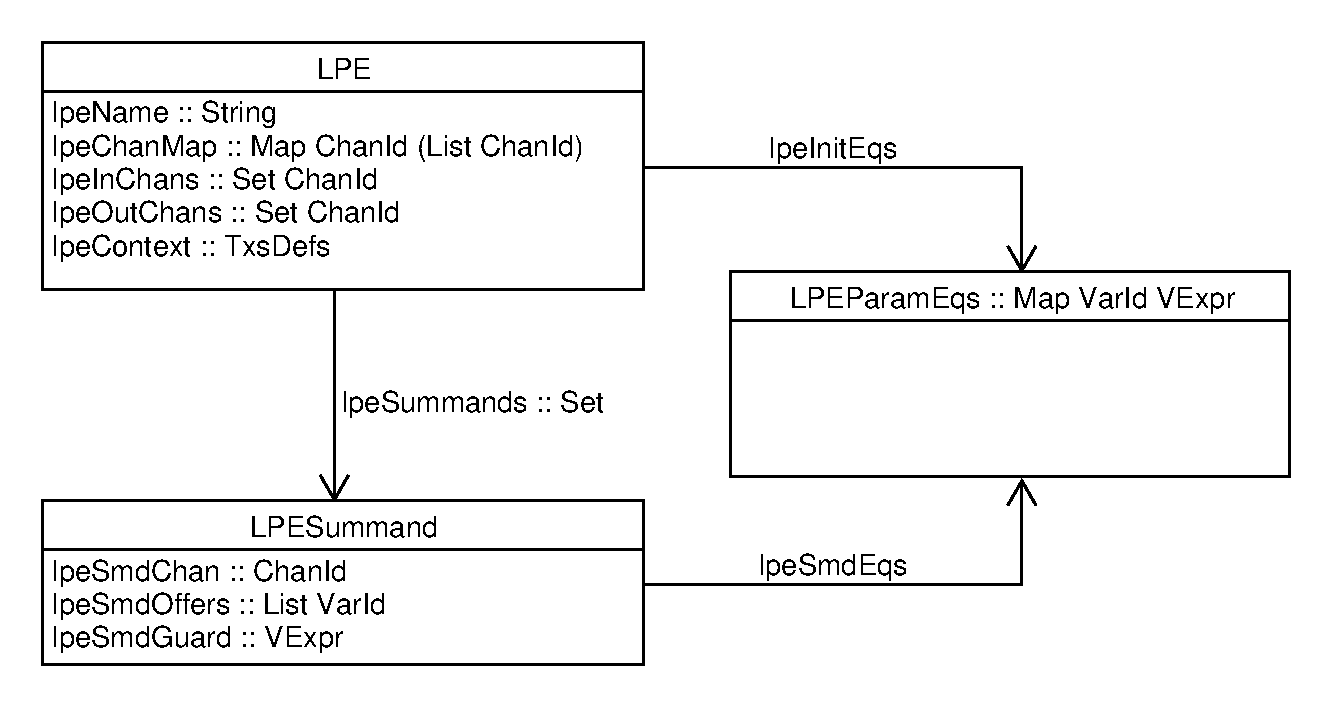
\includegraphics[width=0.7\linewidth]{images/lpe-types}
\caption{LPE data structure.}
\label{lpedatastructure:fig}
\end{center}
\end{figure}

The main data type is \texttt{LPE}.
This type primarily contains information about the \txs{} process in restricted LPE form (see \ref{restrictedlpeform}):
\begin{itemize}
\item The name of the LPE process is \texttt{lpeName};
\item The summands that form the body of the LPE process; and
\item The sorts of the data parameters of the LPE process are contained in \texttt{lpeInitEqs} as well as how each data parameter is initialized.
\end{itemize}

Because the LPE process is always instantiated with the same channels in the same order, the \texttt{LPE} type only has to track which channels are input channels (\texttt{lpeInChans}) and which channels are output channels (\texttt{lpeOutChans}).
Note that these are single channel identifiers that (may) have been freshly generated from multi-channel summands or from summands with hidden variables in order to obtain restricted LPE form (see \ref{restrictedlpeform}).
The \texttt{lpeChanMap} defines how channels in the LPE data structure are converted back to the original channels (it is therefore the implementation of $\Omega_I$ and $\Omega_O$).

The \texttt{LPE} type also stores some circumstantial information in \texttt{lpeContext}.
This is a library of \txs{} type and function definitions that has been copied directly from the original \txs{} model specification.
It is used to validate instances of the \texttt{LPE} type, to generate default values of a specific sort, and more.

Finally, the \texttt{LPESummand} type only contains information about a specific summand: \texttt{lpeSmdChan} is the channel over which it communicates; \texttt{lpeSmdOffers} are the communication variables (including variables that originally were hidden variables); and the \texttt{lpeSmdEqs} map defines which expressions are used to assign new values to the parameters of the LPE after the application of the summand.

\section{Summand elements} \label{summandelements}

To formally reference the elements of $s_i$ -- the $i$th summand of restricted LPE $P$ (see \ref{restrictedlpeform}) -- the following definition is used:
\begin{align*}
s_i = C_i \; \texttt{?} \; x_i(1) \; \cdots{} \; \texttt{?} \; x_i(m_i) \; [[g_i]] \text{ \texttt{>->} } P(v_i(p_1), \cdots{}, v_i(p_k))
\end{align*}

where

\begin{itemize}
\item $C_i$ is the name of the channel over which summand $s_i$ communicates;
\item $m_i \geq 0$ is the number of variables that summand $s_i$ uses to communicate over channel $C_i$;
\item $x_i(j)$ is the $j$th variable that summand $s_i$ uses locally (communication variables first, followed by hidden variables);
\item $g_i$ is the guard of summand $s_i$ (the only free variables in this expression must be parameters of $P$, communication variables of summand $s_i$, or hidden variables of summand $s_i$);
\item $p_1, \cdots{}, p_k$ are the parameters of $P$, of which there are $k \geq 0$;
\item $v_i(p)$ is an expression that defines the new value of parameter $p$ of $P$ after the application of summand $s_i$ (the only free variables in this expression must be LPE parameters, communication variables of summand $s_i$, or hidden variables of summand $s_i$).
\end{itemize}

Note that, because $P$ is in restricted LPE form, the following assumption generally holds for two summands, $s_\alpha$ and $s_\beta$:
\begin{align*}
C_\alpha = C_\beta \rightarrow m_\alpha = m_\beta
\end{align*}


\chapter{step} \label{stepN}

\section{Introduction}

\txs{} provides commands for randomly stepping through a model; however, it may be possible to do this more efficiently when a model is in LPE form.
This hypothesis has been put to the test by developing dedicated stepper functionality.

Early results of the LPE stepper showed equal to worse performance.
The LPE stepper was therefore extended with a preparatory step in which `possible successors' are calculated.
Making use of the extra information, the LPE stepper frequently outperforms the original \txs{} stepper.

\section{Formal background}

\subsection{Possible successors}

Consider summands $s_\alpha$ and $s_\beta$, referencing their elements conform \ref{summandelements}.
Summand $s_\beta$ is said to be a \emph{possible successor} of $s_\alpha$ if the following expression \emph{could be} satisfiable:
\begin{align*}
g_\alpha \land {g_\beta}[v \rightarrow q(v) \;|\; v \in \varsof{g_\beta} \setminus P][p \rightarrow v_\alpha(p) \;|\; p \in P]
\end{align*}

where $q(v)$ is a bijective function that relates variable $v$ to a fresh variable.

\section{Algorithm}

\subsection{Preparation}

The algorithm computes all possible successors for each summand.
(In actuality, the algorithm can compute possible successors of a sequence of summands of arbitrarily chosen length $n \geq 1$.
Unsurprisingly, when choosing $n > 1$ cases in which the costs to compute possible successors are prohibitive are far from uncommon.)

\subsection{Step}

Let $\Sigma$ be a set of tuples $\shPair{\sigma}{h}$ in which $\sigma$ is a model state and $h$ is the history of summands that led to $\sigma$.
Initially, $\Sigma = \{\;\shPair{\sigma_0}{[\;]}\;\}$ where $\sigma_0$ is the initial state as defined by the LPE model.

\subsubsection{1. Compute \istep{}-closure}

Let $T$ be the set of all \istep{} summands of the LPE.
Apply each $t \in T$ to each $\sigma \in \Sigma$.
Any new state $\sigma'$ that is produced by some $t \in T$ is added to $\Sigma$ as $\shPair{\sigma'}{[t]}$.
This is repeated until $\Sigma$ no longer changes.

\subsubsection{2. Find an enabled summand}

Let $\overline{T}$ be the set of all non-\istep{} summands of the LPE.

Consider the summands in $\overline{T}$ in a random order, and let the summand under consideration be $u$.
Determine whether there is a $\shPair{\sigma}{[t]} \in \Sigma$ so that $u$ is enabled when the current state is $\sigma$.
If so, find a \emph{random} variable-to-value mapping $C$ so that $g_u[\; x_u(i) \mapsto C(i) \;|\; i \in [1,\cdots{},m_u] \;]$ holds when the current state is $\sigma$.
Remember $u$ and $C$ (in particular, add it to the random trace that is being constructed) and continue with the next part of the algorithm immediately.

If no $u$ and $C$ can be found, the algorithm reports a deadlock and terminates.

It is also possible that the maximum length of the trace has been reached, in which case the algorithm also terminates.

\subsubsection{3. Determine next states}

In this part of the algorithm, the new value of $\Sigma$ is computed.

For each $\shPair{\sigma}{[t]} \in \Sigma$, look up the possible successors of $t$.
For each possible successor $p$ of $t$, check if the channel of $p$ is the same as the channel of $u$ (that is, if $c_{p} = c_{u}$), then check if $g_p[\; x_p(i) \mapsto C(i) \;|\; i \in [1,\cdots{},m_p] \;]$ holds when the current state is $\sigma$:
\begin{itemize}
\item If the equation holds, apply the summand $p$ to $\sigma$ to find the next state $\sigma'$.
Add $\shPair{\sigma'}{[p]}$ to the new value of $\Sigma$.
\item If the equation does not hold, nothing is added to the new value of $\Sigma$.
\end{itemize}

\clearpage
\section{Benchmark results}

The performance of the LPE stepper has been compared to the performance of the original stepper of \txs{}.
Because the LPE stepper only works for LPEs, the performance of the original stepper has been measured for both unchanged input models and linearized input models.

Figure~\ref{steppers:fig} shows two bars per model: the blue bar is the time that the original stepper of \txs{} required to generate a 100-step trace from the linearized input model as a fraction of $\Delta t$, the time that the original stepper of \txs{} required to generate a 100-step trace from the unchanged input model.
Similarly, the yellow bar is the time that the LPE stepper required to generate a 100-step trace from the linearized input model (obviously, this is a precondition on the input of the LPE stepper) as a fraction of $\Delta t$.
The figure also includes the range of the standard deviation.

\begin{figure}[!ht]
\begin{center}
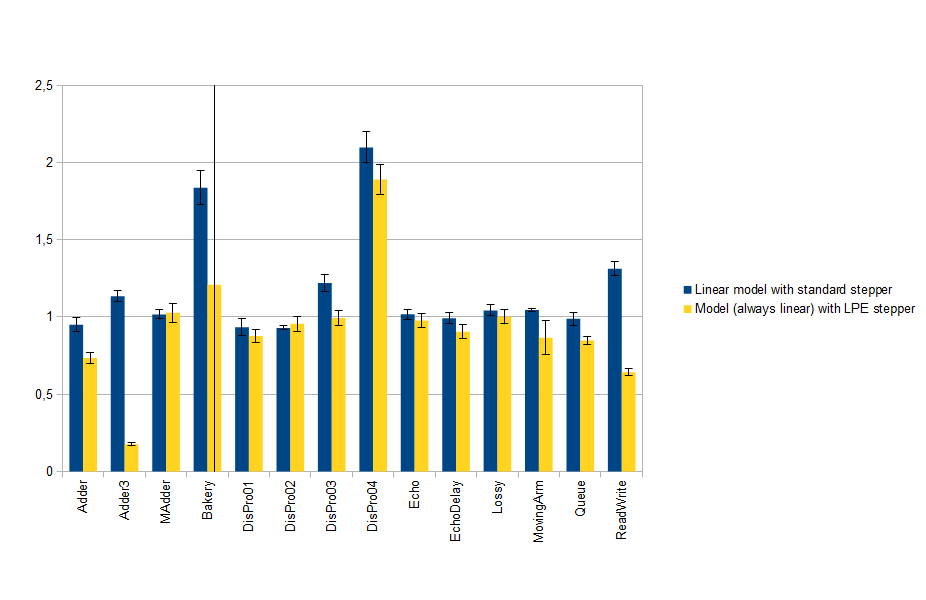
\includegraphics[width=1\linewidth]{charts/steppers-comparison}
\caption{Relative performance of different steppers}
\label{steppers:fig}
\end{center}
\end{figure}

As can be seen in the figure, for 7 out of 14 models the deviation ranges of the measured times overlap, and so we cannot conclude a performance improvement.
For all other models, however, the LPE stepper actually outperforms the original stepper, even though the performance is only impressive for the Adder, Adder3, and ReadWrite models.

The Bakery model has a very large standard deviation.
This deviation results from the long preparatory step that the model requires -- it is quite a large model -- and from the way in which benchmark measurements were taken:
\begin{enumerate}
\item The LPE stepper was instructed to generate a 100-step trace.
The required time $\Delta t _ {100}$ was measured.
\item The LPE stepper was instructed to generate a 0-step trace.
The required time $\Delta t _ {0}$ was measured.
\item $\Delta t$ was computed by subtracting $\Delta t _ {0}$ from $\Delta t _ {100}$.
\end{enumerate}
Naturally, the impact of the deviation in $\Delta t _ {0}$ becomes stronger as the value of $\Delta t _ {0}$ increases relative to $\Delta t _ {100} - \Delta t _ {0}$.


\chapter{clean} \label{clean}

\section{Introduction}

An LPE may contain redundant information, for example because some of its summands contain all behavior of other summands or because some of its summands will never be (or become) enabled.
Obviously, such summands can be removed without hesitation, which may result in a speedup in other computations in which the LPE is input.

The \texttt{clean} command attempts to detect redundant summands and removes the ones that it finds.
The state space of the LPE is not affected by the changes.

\section{Formal background}

\subsection{Summand containment}

Consider two summands, $s_\alpha$ and $s_\beta$, and reference their elements conform \ref{summandelements}.

Summand $s_\alpha$ is said to \emph{contain} $s_\beta$ if these two conditions hold:

\begin{itemize}
\item $s_\alpha$ and $s_\beta$ must communicate over the exact same channel with exactly as many channel variables; that is, $C_\alpha = C_\beta \land m_\alpha = m_\beta$.

\item Define the mapping
\begin{align*}
X_\alpha = [x_\beta(j) \rightarrow x_\alpha(j) \;|\; 1 \leq j \leq \text{min}(m_1, m_2)]
\end{align*}

The following conditions must also hold:
\begin{align*}
g_\beta[X_\alpha] &\rightarrow g_\alpha \\
v_\alpha(p) = v_\beta(p)[X_\alpha] &\leftrightarrow \text{\textit{True}} \text{ for all } p \in [p_1, \cdots{}, p_k]
\end{align*}

The first condition demands that whenever $s_\beta$ is enabled, $s_\alpha$ must also be enabled; consequently, $s_\alpha$ is `always ready' to perform the same behavior as $s_\beta$.
The second condition demands that the state after the application of $s_\alpha$ is the same as the state after the application of $s_\beta$, regardless of the values of communication variables and LPE parameters.
\end{itemize}

Note that $s_\alpha$ could contain all behavior of $s_\beta$ without these two conditions being true (we under-approximate by tolerating false negatives)!

\subsection{Summand reachability}

Consider summands $s_\alpha$ and $s_\beta$, referencing their elements conform \ref{summandelements}.
Summand $s_\alpha$ is said to be a \emph{possible predecessor} of $s_\beta$ if the following expression \emph{could be} satisfiable:
\begin{align*}
g_\alpha \land {g_\beta}[v \rightarrow q(v) \;|\; v \in \varsof{g_\beta} \setminus P][p \rightarrow v_\alpha(p) \;|\; p \in P]
\end{align*}

where $q(v)$ is a bijective function that relates variable $v$ to a fresh variable.

A summand $s_\beta$ is said to be \emph{reachable} if at least one of these conditions holds:

\begin{itemize}
\item It is possible that summand $s_\beta$ is enabled in the initial state of the LPE.
Formally, $s_\beta$ is reachable if the LPE is initialized as
\begin{align*}
P(v_I(p_1), \cdots{}, v_I(p_m))
\end{align*}

and if
\begin{align*}
g_\beta[p \rightarrow v_I(p) \;|\; p \in P]
\end{align*}

\emph{could be} satisfiable.

\item There exists at least one other summand $s_\alpha$ in the same LPE that is a possible predecessor of $s_\beta$.
It is \emph{not} sufficient if the only possible predecessor of $s_\beta$ is $s_\beta$ itself!
\end{itemize}

Summand reachability is \emph{over-approximated}.
For example, if it is uncertain whether a summand is enabled in the initial state, the summand is considered to be reachable.

\section{Algorithm}

The algorithm consists of 2 phases.

In the first phase, the algorithm does a pairwise comparison of all summands of the LPE.
If it discovers that some summand $s_1$ contains another summand $s_2$, it removes $s_2$ from the LPE.

In the second phase, the algorithm starts by determining which summands are reachable in the initial state of the LPE (the first condition for reachability in the previous section).
This becomes the initial value of the set $X$.
Then, until a fixpoint is reached, to $X$ all summands are added of which there exists a possible predecessor in $X$.
The output LPE of the algorithm contains all summands that are in the fixpoint of $X$.

\section{Example}

Consider the following LPE:

\begin{lstlisting}
//Process definition:
PROCDEF example[A :: Int](x :: Int)
  = A ? i [[x==0]] >-> example[A](1)
  + A ? j [[x==1]] >-> example[A](2)
  + A ? k [[x==1]] >-> example[A](2)
  + A ? l [[x==2]] >-> example[A](0)
  + A ? m [[x>=2]] >-> example[A](0)
  ;

//Initialization:
example[A](0);
\end{lstlisting}

The \texttt{clean} command will detect that the second and third summands of the LPE are equivalent and remove one of them.
It will also detect that the fifth summand contains the fourth summand, and therefore remove the fourth summand.

Now consider

\begin{lstlisting}
//Process definition:
PROCDEF example[A :: Int, B](x :: Int)
  = A ? i [[i != 13]] >-> example[A, B](i)
  + B [[x == 13]] >-> example[A, B](x)
  ;

//Initialization:
example[A, B](0);
\end{lstlisting}

The second summand is unreachable: it is not enabled in the initial state (since \texttt{x = 0}) and it is never enabled after the application of the first summand (since \texttt{i != 13}).

\section{Benchmark results}

The following durations were measured with a benchmark for several models:
\begin{itemize}
\item The average duration of \txs{} to make 500 steps in a model without converting it to LPE form or applying LPE operations;
\item The average duration of \txs{} to make 500 steps in a model after it has been converted to LPE form;
\item The average duration of \txs{} to make 500 steps in a model after it has been converted to LPE form and after the \texttt{clean} operation has been applied.
\end{itemize}

When plotting the second series of measurements against the first (see Figure~\ref{lpe-only-vs-original:fig}), the following conclusions can be drawn:
\begin{itemize}
\item The effect of the LPE transformation on performance is negative in most cases.
\item The effect of the LPE transformation on performance is positive in some cases, but not dramatically so.
\item For one model (\texttt{Adder3}), the effect of the LPE transformation is extremely positive (5.2 seconds instead of 12.5).
Unfortunately, this model is not very realistic since it simply consists of three parallel processes without any synchronization.
\end{itemize}

\begin{figure}[!ht]
\begin{center}
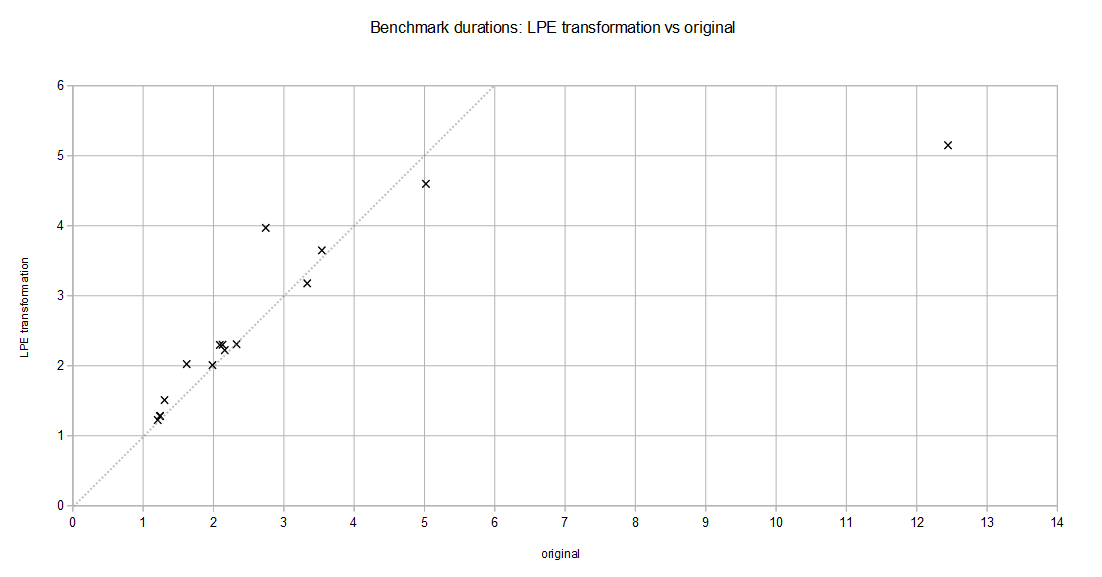
\includegraphics[width=0.8\linewidth]{charts/lpe-only-vs-original}
\caption{Benchmark results: LPE transformation vs original}
\label{lpe-only-vs-original:fig}
\end{center}
\end{figure}

It is possible that the \texttt{clean} operation has a significant positive influence on the performance of \txs{}.
Based on a plot of the third series of measurements against the second (see Figure~\ref{clean-vs-lpe-only:fig}), however, this cannot be concluded: only part of the models show slight (but significant) improvements, whereas other models suffer an (also slight) additional performance loss.

\begin{figure}[!ht]
\begin{center}
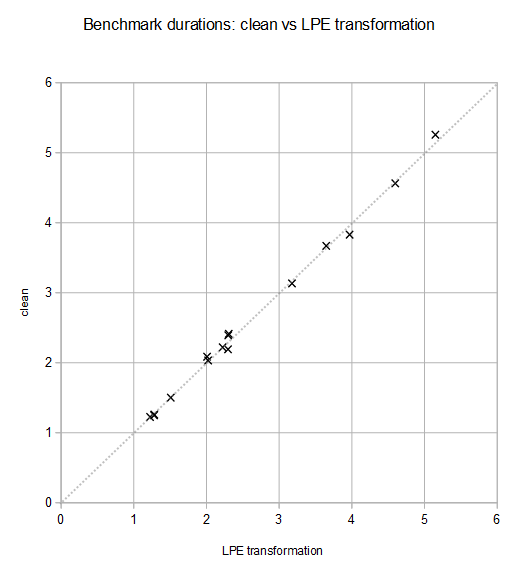
\includegraphics[width=0.5\linewidth]{charts/clean-vs-lpe-only}
\caption{Benchmark results: clean vs LPE transformation}
\label{clean-vs-lpe-only:fig}
\end{center}
\end{figure}




\chapter{cstelm}

\section{Introduction}

An LPE may have parameters that do not change value throughout the state space of that process.
These parameters are essentially \emph{constant}.
Removing constant parameters results in a smaller state vector (which may improve performance), but otherwise the state space of an LPE remains the same.

Constants can be safely removed from a process as follows:
\begin{enumerate}
\item Substitute references to a constant parameter by the initial (explicit) value of that parameter;
\item Remove the constant from the process parameter list.
\end{enumerate}

\section{Algorithm}

The algorithm consists of the following steps \cite{groote2001computer}:

\begin{enumerate}

\item Make it so that all LPE parameters are \labeledas{constant}.

\item Let $X$ be the set of all LPE parameters that are \labeledas{constant}.
Define a substitution $V = [p \rightarrow v_I(p) \;|\; p \in X]$, where $v_I(p)$ gives the initial value of LPE parameter $p$.

\item Consider each summand $s$ of the LPE.
Construct an equation $g_s \rightarrow p = v_s(p)$ for all $p \in X$, where $g_s$ is the guard of $s$ and where $v_s(p)$ is the expression that defines the value of LPE parameter $p$ after the application of summand $s$, and apply the substitution $V$ to it.
(This gives $(g_s \rightarrow p = v_s(p))[V] \Leftrightarrow {g_s}[V] \rightarrow v_I(p) = v_s(p)[V]$.)

If the obtained equation is a tautology (that is, if its negation is unsatisfiable) for all $s$, $p$ remains \labeledas{constant}; otherwise, \removelabelfrom{constant} $p$.

\item Repeat the previous two steps until the fixpoint of $X$ is reached.
Then remove all LPE parameters that are still \labeledas{constant} from the LPE, substituting references to those parameters by their initial values.

\end{enumerate}

\section{Example}

Consider the following LPE:

\begin{lstlisting}
//Process definition:
PROCDEF example[A](x, y, z :: Int)
  = A [[z = 2]] >-> example[A](z-1, 1, 2)
  + A >-> example[A](y, x, x+y)
  + A >-> example[A](1, x, z+1)
  ;

//Initialization:
example[A](1, 1, 2);
\end{lstlisting}

First, $V = [ x \rightarrow 1, y \rightarrow 1, z \rightarrow 2 ]$.

We must check the following equations:

\begin{align*}
(z = 2 \rightarrow x = z-1)[V] &\Leftrightarrow (2 = 2 \rightarrow 1 = 2-1) \Leftrightarrow \textit{true} \\
(z = 2 \rightarrow y = 1)[V] &\Leftrightarrow (2 = 2 \rightarrow 1 = 1) \Leftrightarrow \textit{true} \\
(z = 2 \rightarrow z = 2)[V] &\Leftrightarrow (2 = 2 \rightarrow 2 = 2) \Leftrightarrow \textit{true} \\
(x = y)[V] &\Leftrightarrow (1 = 1) \Leftrightarrow \textit{true} \\
(y = x)[V] &\Leftrightarrow (1 = 1) \Leftrightarrow \textit{true} \\
(z = x+y)[V] &\Leftrightarrow (2 = 1+1) \Leftrightarrow \textit{true} \\
(x = 1)[V] &\Leftrightarrow (1 = 1) \Leftrightarrow \textit{true} \\
(y = x)[V] &\Leftrightarrow (1 = 1) \Leftrightarrow \textit{true} \\
(z = z+1)[V] &\Leftrightarrow (2 = 2+1) \Leftrightarrow \textit{false} \\
\end{align*}

The last equation is not a tautology, and the `constant' label is therefore removed from $z$.

The new value of $V$ is $[ x \rightarrow 1, y \rightarrow 1 ]$.

\clearpage
The equations are now the following:

\begin{align*}
(z = 2 \rightarrow x = z-1)[V] &\Leftrightarrow (z = 2 \rightarrow 1 = z-1) \Leftrightarrow \textit{true} \\
(z = 2 \rightarrow y = 1)[V] &\Leftrightarrow (z = 2 \rightarrow 1 = 1) \Leftrightarrow \textit{true} \\
(x = y)[V] &\Leftrightarrow (1 = 1) \Leftrightarrow \textit{true} \\
(y = x)[V] &\Leftrightarrow (1 = 1) \Leftrightarrow \textit{true} \\
(x = 1)[V] &\Leftrightarrow (1 = 1) \Leftrightarrow \textit{true} \\
(y = x)[V] &\Leftrightarrow (1 = 1) \Leftrightarrow \textit{true} \\
\end{align*}

All of the equations above are tautologies, and so $x$ and $y$ remain labeled with `constant'.
A fixpoint has been reached; removing $x$ and $y$ from the LPE gives

\begin{lstlisting}
//Process definition:
PROCDEF example[A](z :: Int)
  = A [[z==2]] >-> example[A](2)
  + A [[true]] >-> example[A](2)
  + A [[true]] >-> example[A](z+1)
  ;

//Initialization:
example[A](2);
\end{lstlisting}

Obviously, more simplification is possible.
Applying the \texttt{clean} command (see \ref{clean}) gives

\begin{lstlisting}
//Process definition:
PROCDEF example[A](z :: Int)
  = A [[true]] >-> example[A](2)
  + A [[true]] >-> example[A](z+1)
  ;

//Initialization:
example[A](2);
\end{lstlisting}

\section{Benchmark results}

The following durations were measured with a benchmark for several models:
\begin{itemize}
\item The average duration of \txs{} to make 500 steps in a model after it has been converted to LPE form;
\item The average duration of \txs{} to make 500 steps in a model after it has been converted to LPE form and after the \texttt{cstelm} operation has been applied.
\end{itemize}

When plotting the second series of measurements against the first (see Figure~\ref{cstelm-vs-lpe-only:fig}), it becomes clear that the effect of \texttt{cstelm} is tiny.

\begin{figure}[!ht]
\begin{center}
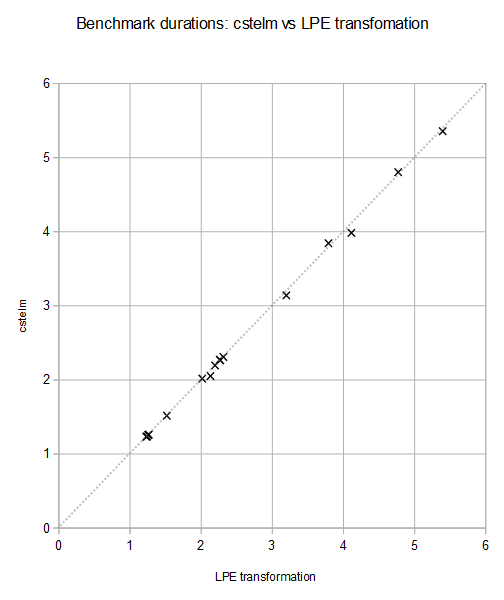
\includegraphics[width=0.7\linewidth]{charts/cstelm-vs-lpe-only}
\caption{Benchmark results: cstelm vs LPE transformation}
\label{cstelm-vs-lpe-only:fig}
\end{center}
\end{figure}


\chapter{parelm}

\section{Introduction}

An LPE may have parameters that do not affect the behavior of that process in any way.
These parameters are said to be \emph{inert}.
Removing inert parameters from an LPE reduces the size of state vectors and the state space of that LPE, which both benefits performance.

\section{Algorithm}

The algorithm consists of the following steps \cite{groote2001computer}:

\begin{enumerate}

\item Make it so that all parameters of the LPE are \labeledas{inert}.

\item Consider the guards of all summands of the LPE, and \removelabelfrom{inert} from all LPE parameters that occur in the guard of a summand.

\item Let $X$ be the set of all LPE parameters that are \labeledas{inert}, and consider all expressions $v_s(p)$ that define the value of an LPE parameter $p$ after application of a summand $s$.
For each such expression, if $p$ is \emph{not} \labeledas{inert}, \removelabelfrom{inert} all LPE parameters that occur in $v_s(p)$.

\item Repeat the previous step until the fixpoint of $X$ is reached.
Then remove all LPE parameters that are still \labeledas{inert} from the LPE, substituting references to those parameters by their initial values.

\end{enumerate}

\clearpage
\section{Example}

Consider the following LPE:

\begin{lstlisting}
//Process definition:
PROCDEF example[A :: Int, B](x, y, z :: Int)
  = A ? i [[x==0]] >-> example[A, B](i, y, z)
  + A ? i [[x==1]] >-> example[A, B](0, i, z)
  + B [[x==2]] >-> example[A, B](0, y, z)
  + B [[true]] >-> example[A, B](z, y, x)
  ;

//Initialization:
example[A, B](0, 0, 0);
\end{lstlisting}

First, the `inert' label is removed from $x$ because $x$ occurs in the guards of the first three summands.

In the fourth summand, $z$ is used in the expression of which the value is assigned to $x$.
Therefore $z$ is also no longer \labeledas{inert}.

$y$ remains labeled with `inert': it does not occur in a guard, nor is it used in the assignment to a process parameter other than itself.
Removing $y$ gives

\begin{lstlisting}
//Process definition:
PROCDEF example[A :: Int, B](x, z :: Int)
  = A ? i [[x==0]] >-> example[A, B](i, z)
  + A ? i [[x==1]] >-> example[A, B](0, z)
  + B [[x==2]] >-> example[A, B](0, z)
  + B [[true]] >-> example[A, B](z, x)
  ;

//Initialization:
example[A, B](0, 0);
\end{lstlisting}

\section{Benchmark results}

The following durations were measured with a benchmark for several models:
\begin{itemize}
\item The average duration of \txs{} to make 500 steps in a model after it has been converted to LPE form;
\item The average duration of \txs{} to make 500 steps in a model after it has been converted to LPE form and after the \texttt{parelm} operation has been applied.
\end{itemize}

When plotting the second series of measurements against the first (see Figure~\ref{parelm-vs-lpe-only:fig}), it is easy to see that the impact is insignificant in most cases.
The only model for which a significant performance increase has been measured is the \texttt{ControlLoop} model, which has indeed lost part of its state vector.

\begin{figure}[!ht]
\begin{center}
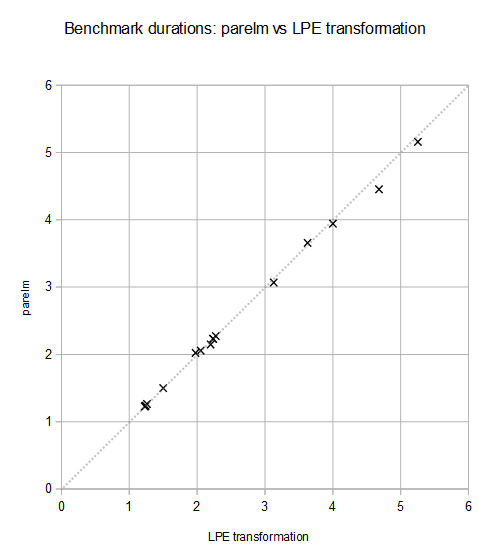
\includegraphics[width=0.5\linewidth]{charts/parelm-vs-lpe-only}
\caption{Benchmark results: parelm vs LPE transformation}
\label{parelm-vs-lpe-only:fig}
\end{center}
\end{figure}


\chapter{parreset}

\section{Introduction}

An LPE may have parameters of which the values are not used anymore after a particular state.
If such parameters can have different values after that state, they continue to add states to the state space for each of those values -- \emph{without} adding any new behavior!

The \texttt{parreset} command tries to determine whether the value of a parameter is used by an LPE after a particular summand.
If this is the case, the parameter is said to be \emph{relevant} for that summand; otherwise, the summand can `reset' the parameter, meaning that it can be assigned a default value.

To determine the relevance of parameters, \texttt{parreset} analyzes the reachability of summands in a generalized, symbolic manner.
The \texttt{datareset} command, serving a similar purpose (see \ref{datareset}), does a control-flow analysis instead.

\section{Formal background}

\subsection{Possible successors} \label{possiblesuccessors}

Consider summands $s_\alpha$ and $s_\beta$, referencing their elements conform \ref{summandelements}.
Summand $s_\beta$ is said to be a \emph{possible successor} of $s_\alpha$ if the following expression \emph{could be} satisfiable:
\begin{align*}
g_\alpha \land {g_\beta}[v \rightarrow q(v) \;|\; v \in \varsof{g_\beta} \setminus P][p \rightarrow v_\alpha(p) \;|\; p \in P]
\end{align*}

where $q(v)$ is a bijective function that relates variable $v$ to a fresh variable.

\section{Algorithm}

The algorithm is a generalization of an existing algorithm \cite{van2009state}.
It consists of two phases.

During the first phase (the preparation phase), we determine all successors of each summand of the LPE using the equation from the previous section.

The second phase (the iteration phase) follows these steps:

\begin{enumerate}

\item For each summand $s_\alpha$ of the LPE, create a set $R_\alpha$ that contains all parameters of the LPE.
This means that, initially, we assume that all parameters of the LPE are used by one or more of the successors of $s_\alpha$; that is, \emph{relevant} to $s_\alpha$.

\item For each summand $s_\alpha$ of the LPE, set the value of $R_\alpha$ to $\bigcup\limits_{s_\beta \in S_\alpha}^{} r(s_\beta)$ where $S_\alpha$ is the set of all successors of $s_\alpha$ (as determined during the preparation phase) and where $r$ is the function
\begin{align*}
r(s_\beta) = \left( \text{vars}(g_\beta) \cup \bigcup\limits_{x \in R_\beta}^{} \text{vars}(v_\beta(x)) \right) \setminus C_\beta
\end{align*}

\item Repeat the previous step until the fixpoint of $R_\alpha$ is reached for each summand $s_\alpha$ of the LPE.

\item For each summand $s_\alpha$ and for all $p \in P \setminus R_\alpha$, change the expression $v_\alpha(p)$ (which defines the value of LPE parameter $p$ after the application of $s$) to $v_I(p)$, the value of $p$ in this initial state of the LPE.

\end{enumerate}

\section{Example}

Consider the following LPE:

\begin{lstlisting}
//Process definition:
PROCDEF example[A :: Int, B](x, y :: Int)
  = A ? i [[x==0]] >-> example[A, B](1, i)
  + A ? i [[x==1 && i==y]] >-> example[A, B](2, y)
  + B [[x==2]] >-> example[A, B](3, y)
  + B [[x==3]] >-> example[A, B](0, y)
  ;

//Initialization:
example[A, B](0, 0);
\end{lstlisting}

Let the summands be represented by $s_1$ from $s_4$ (from top to bottom).

Finding the successors of each summand is easy: each summand has exactly one successor, namely the next one, except in case of $s_4$, where the $s_1$ is the successor.

It is also obvious that $x$ will always be in $R_\alpha$ for each summand $s_\alpha$, because each summand $s_\alpha$ uses $x$ in its guard.

Process parameter $y$ will always be in $R_1$ because $y$ is used in the guard of $s_1$'s successor, $s_2$.
After a few iterations, however, $y$ is removed from $R_2$, $R_3$, and $R_4$.
This means that $y$ is assigned a default value in $s_2$, $s_3$, and $s_4$.
Choosing the initial value of $y$ as its default value gives

\begin{lstlisting}
//Process definition:
PROCDEF example[A :: Int, B](x, y :: Int)
  = A ? i [[x==0]] >-> example[A, B](1, i)
  + A ? i [[x==1 && i==y]] >-> example[A, B](2, 0)
  + B [[x==2]] >-> example[A, B](3, 0)
  + B [[x==3]] >-> example[A, B](0, 0)
  ;

//Initialization:
example[A, B](0, 0);
\end{lstlisting}

\section{Benchmark results}

The following durations were measured with a benchmark for several models:
\begin{itemize}
\item The average duration of \txs{} to make 500 steps in a model after it has been converted to LPE form;
\item The average duration of \txs{} to make 500 steps in a model after it has been converted to LPE form and after the \texttt{parreset} operation has been applied.
\end{itemize}

When plotting the second series of measurements against the first (see Figure~\ref{parreset-vs-lpe-only:fig}), it is easy to see that the impact is insignificant in most cases.

\begin{figure}[!ht]
\begin{center}
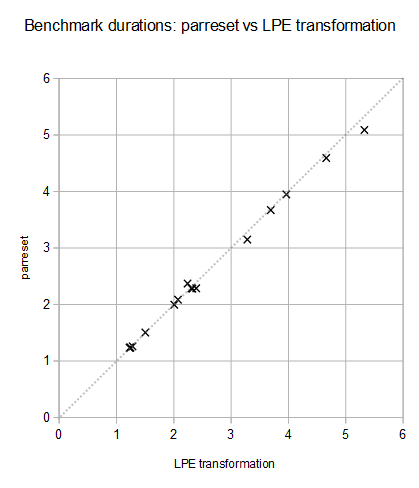
\includegraphics[width=0.7\linewidth]{charts/parreset-vs-lpe-only}
\caption{Benchmark results: parreset vs LPE transformation}
\label{parreset-vs-lpe-only:fig}
\end{center}
\end{figure}



\chapter{datareset} \label{datareset}

\section{Introduction}

The \texttt{datareset} command assumes that certain parameters of the LPE determine which summands can be followed by which summands.
These parameters determine the control-flow of the LPE, and are therefore called \emph{control-flow parameters}.

\emph{Data parameters}, on the other hand, are used to store values, and often temporarily, which means that their values may not be used anymore after a particular state.
Data parameters can typically have different values after such a state, which causes them to add states to the state space for each of those values -- \emph{without} adding any new behavior!

The \texttt{datareset} command attempts to detect LPE control-flows and determine the parts of those control-flows where data parameters are no longer used.
At these locations, data parameters are set to a default value (`reset').
This removes states from the state space, potentially improving performance of subsequent computations.

\section{Formal background}

The control-flow analysis is based on work done in \cite{van2009state}.

\subsection{Parameter properties}

Each parameter $p$ of a summand $s$ has the following properties:
\begin{itemize}

\item Is the value of $p$ potentially altered by $s$?
If so, $p$ receives the label `changed'.

\item Does $p$ occur in the guard of $s$?
If so, $p$ receives the label `directly used'.

\item Has $p$ received the label `directly used' in $s$?
Or does $p$ occur in the assignment by $s$ to a parameter that has received the label as `changed'?
In either case, $p$ also receives the label `used'.

\item Must the value of $p$ have a specific (unique) value $v$ in order for $s$ to be enabled?
If so, $p$ receives the label `having a source' for $s$, with the source being $v$.

\item Does the value of $p$ have a specific (unique) value $v$ immediately after $s$ has been applied?
If so, $p$ receives the label `having a destination' for $s$, with the source being $v$.

\item Does $p$ have both a source and a destination for $s$?
Then $p$ is called a \emph{ruling parameter}, and $p$ is said to `rule' summand $s$.

\end{itemize}

\subsection{Control-flow graphs}

A parameter of the LPE is a \emph{control-flow parameter} of the LPE if for all summands it is either a ruling parameter or not \labeledas{changed} (or both).
A parameter that is not a control-flow parameter is defined as a \emph{data parameter}.

\vspace{1mm}

For each control-flow parameter $f$ of the LPE, a control-flow graph is constructed.
There is a state in the control-flow graph for each source and destination of $f$ (across all summands).
Two states $s_1$ and $s_2$ are connected by an edge $(s_1, i, s_2)$ if there is a summand $i$ where the source of $f$ is represented by one of the states and where the destination of $f$ is represented by the other state.
The direction of such an edge is from source state to destination state.

\subsection{Belongs-to function}

Here, the \emph{belongs-to} function is introduced.
The belongs-to function maps each data parameter $d$ to some set of control-flow parameters $b(d)$ as follows

\begin{align*}
b(d) = F \cap \bigcap\limits_{s \in S}^{} \text{ruling}(s)
\end{align*}

where

\begin{itemize}
\item $F$ is the set of all control-flow parameters;
\item $S$ is the set of all summands in which $d$ is \labeledaseither{changed}{used};
\item $\text{ruling}(s)$ is the set of all parameters that rule summand $s$.
\end{itemize}

\section{Algorithm}

The algorithm executes 3 phases: the preparatory phase, the iterative phase, and the deletion phase.

\subsection{Preparatory phase}

In this phase, the parameter properties, control-flow graphs and belongs-to function are computed.

\subsection{Iterative phase}

In the iterative phase, the so-called \emph{relevance relation} is computed.
This relation, with symbol $R$, relates a data parameter $d$, a control-flow parameter $f$, and a value $v$ if $d$ is `relevant' after a state in which $f$ has value $v$.
This is denoted $R(d, f, v)$.
Intuitively, this is a situation in which $d$ should \emph{not} be reset because its value may be needed in the future.

The computation of $R$ is a fixpoint algorithm: modifications are applied iteratively until $R$ no longer changes.
The initial value of $R$ is set to
\begin{align*}
R_0 = \bigcup\limits_{\substack{i \in S \\ d_k \in \text{directlyUsed}(i)}}^{} \;\{\; (d_k, d_j, \text{source}(i, d_j)) \;|\; d_j \in b(d_k) \;\}
\end{align*}

where

\begin{itemize}
\item $S$ is the set of all summands;
\item $\text{directlyUsed}(i)$ is a function that gives the set of all parameters that are \labeledas{directly used} in a summand $i$;
\item $\text{source}(i, f)$ is a function that gives the source value of a control-flow parameter $f$ for a summand $i$.
\end{itemize}

Each iteration can be split into two steps.
The first step checks for control-flow graphs in which a data parameter $d$ has already been \labeledas{relevant} whether this implies that $d$ is also relevant in preceding states (of the same control-flow graph).
If so, the appropriate triples are added to $R$:
\begin{align*}
R_{n}{'} = R_{n-1} \cup \bigcup\limits_{\substack{i \in S}}^{} \;\left\{\; (d_k, d_j, s) \;\middle|\; \substack{(d_l, d_j, t) \in R_{n-1} \\ d_j \in b(d_k) \\ d_k \in \text{vars}(v_i(d_l)) \\ (s, i, t) \in E_{d_j}} \;\right\}
\end{align*}

where

\begin{itemize}
\item $E_{f}$ is the set of edges that are part of the control-flow graph of control-flow parameter $f$.
\end{itemize}

The second step is similar, but data parameters that are found to be relevant are added as triples to $R$ in relation to \emph{another} control-flow parameter:
\begin{align*}
R_{n} = R_{n}{'} \cup \bigcup\limits_{\substack{i \in S}}^{} \;\left\{\; (d_k, d_j, \text{source}(i, d_j)) \;\middle|\; \substack{(d_l, d_p, t) \in R_{n}{'} \\ d_j \in b(d_k),\; d_j \notin b(d_l) \\ d_k \in \text{vars}(v_i(d_l)) \\ (r, i, t) \in E_{d_p}} \;\right\}
\end{align*}

\subsection{Deletion phase}

Finally, each summand of an LPE is subject to modification.
Modifications are made by making use of the belongs-to function $b$ and the relevance relation $R$.
Intuitively, we check whether the value of a parameter is `relevant' after a specific summand $i$ has been applied.
If so, the parameter should not be reset.
Otherwise, the parameter can be reset, for example to its initialization value:

\begin{align*}
v_{i}{'}(d_k) = \begin{cases}
v_{i}(d_k) & \text{if } \bigwedge\limits_{\substack{d_j \in \text{ruling}(i) \\ d_j \in b(d_k)}}^{} R(d_k, d_j, \text{dest}(i, d_j)) \\
v_{I}(d_k) & \text{otherwise}
\end{cases}
\end{align*}

where

\begin{itemize}
\item $\text{ruling}(s)$ is the set of all parameters that rule summand $s$;
\item $\text{source}(i, f)$ is a function that gives the destination value of a control-flow parameter $f$ for a summand $i$.
\end{itemize}

\section{Benchmark results}

The following durations were measured with a benchmark for several models:
\begin{itemize}
\item The average duration of \txs{} to make 500 steps in a model after it has been converted to LPE form;
\item The average duration of \txs{} to make 500 steps in a model after it has been converted to LPE form and after the \texttt{datareset} operation has been applied.
\end{itemize}

When plotting the second series of measurements against the first (see Figure~\ref{datareset-vs-lpe-only:fig}), it is easy to see that the impact is insignificant in most cases.

\begin{figure}[!ht]
\begin{center}
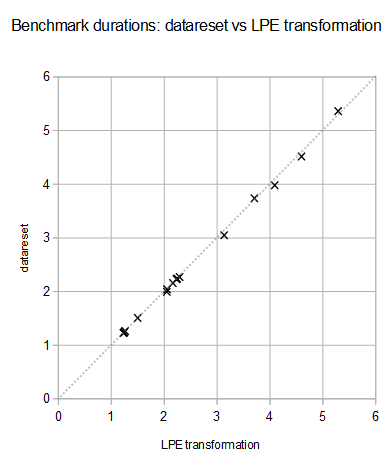
\includegraphics[width=0.7\linewidth]{charts/datareset-vs-lpe-only}
\caption{Benchmark results: datareset vs LPE transformation}
\label{datareset-vs-lpe-only:fig}
\end{center}
\end{figure}


\chapter{confcheck} \label{confcheck}

\section{Introduction}

The \texttt{confcheck} command perform a \emph{confluence analysis} on the LPE in order to determine which \istep{} summands are \emph{confluent}
A confluent \istep{} summand is an \istep{} summand with the property that the possible behavior of a system is the same up to branching bisimulation before and after the application of that summand.

The \texttt{confcheck} command will rename confluent \istep{}s to \cistep{}s.
Afterwards, the \texttt{confelm} command can be used next in order to prioritize \cistep{}s, which may reduce the state space.

\section{Algorithm}

Consider all possible summands pairs, referencing the elements of the summands conform \ref{summandelements}.
Select all pairs $(s_\alpha, s_\beta)$ of which $C_\alpha$ equals \istep{}.

Since it cannot be assumed that
\begin{align*}
\{ x_1(1), \cdots{} x_1(m_1) \} \cap \{ x_2(1), \cdots{} x_2(m_2) \} = \emptyset{}
\end{align*}

a substitution $X$ is introduced such that
\begin{align*}
X = [ x_2(j) \rightarrow q(x_2(j)) \;|\; 1 \leq j \leq m_2 ]
\end{align*}

where $q(x)$ is a surjective function that yields fresh variables.

We also define
\begin{align*}
V_{1} &= [p_j \rightarrow v_1(p_j) \;|\; 1 \leq j \leq k] \\
V_{2} &= [p_j \rightarrow v_2(p_j)[X] \;|\; 1 \leq j \leq k]
\end{align*}

Using the definitions above, a particular \istep{} summand $s_1$ is confluent if the following expression is a tautology for all pairs $(s_1, s_2)$ such that $s_2 \neq s_1$:
\begin{align*}
g_1 \land g_2[X] \rightarrow g_1[V_2] \land g_2[X][V_1] \land \bigwedge\limits_{j=1}^{k} p_j[V_2][V_1] = p_j[V_1][V_2]
\end{align*}

Note that this approach does \emph{not} yield all confluent \istep{} summands (it is an under-approximation).

\section{Example}

Consider the following example:

\begin{lstlisting}
//Process definition:
PROCDEF example[A :: Int](x, y :: Int)
  = A ? i [[x<=9 /\ x==i]] >-> example[A](x+1, y)
  + ISTEP [[y<=9]] >-> example[A](x, y+1)
  ;

//Initialization:
example[A](0, 0);
\end{lstlisting}

Let $s_1$ be the first and $s_2$ the second summand.
Is $s_2$ confluent?

First, since $\{ x_1(1), \cdots{} x_1(m_1) \} \cap \{ x_2(1), \cdots{} x_2(m_2) \} = \emptyset{}$, $X$ can be ignored.

Second, if
\begin{align*}
g_1 \land g_2 \Leftrightarrow (x \leq 9 \land x=i) \land (y \leq 9)
\end{align*}

holds, then
\begin{align*}
g_1[V_2] \land g_2[V_1] &\Leftrightarrow (x \leq 9 \land x=i)[ y \rightarrow y+1 ] \land (y \leq 9)[ x \rightarrow y+1 ] \\
&\Leftrightarrow (x \leq 9 \land x=i) \land (y \leq 9)
\end{align*}

holds as well.

Third, it is the case that
\begin{align*}
x[V_1][V_2] = x+1 = x[V_2][V_1] \\
y[V_1][V_2] = y+1 = y[V_2][V_1]
\end{align*}

Therefore the confluence condition holds, which means that $s_2$ is confluent.

To store the new information about the second summand, the channel is renamed to \cistep{}:

\begin{lstlisting}
//Process definition:
PROCDEF example[A :: Int](x, y :: Int)
  = A ? i [[x<=9 /\ x==i]] >-> example[A](x+1, y)
  + CISTEP [[y<=9]] >-> example[A](x, y+1)
  ;

//Initialization:
example[A](0, 0);
\end{lstlisting}


\chapter{confelm}

\section{Introduction}
One way in which information about confluence can be used before state space generation, is by appending confluent ISTEPs to other summands.
This has the effect that other branches that could follow those summands are ignored, reducing the size of the state space while maintaining its equivalence up to branching bisimulation.

\section{Formal background}

\subsection{Definite successors}

Consider a summand pair $(s_\alpha, s_\beta)$, referencing the elements of $s_\alpha$ and $s_\beta$ conform \ref{summandelements}.
Summand $s_\beta$ is said to be a \emph{definite successor} of $s_\alpha$ if the following expression is a tautology:
\begin{align*}
g_\alpha \rightarrow {g_\beta}[v \mapsto q(v) \;|\; v \in \varsof{g_\beta} \setminus P][p \mapsto v_\alpha(p) \;|\; p \in P]
\end{align*}

where $q(v)$ is a bijective function that relates variable $v$ to a fresh variable.

For a summand $s$, let $D(s)$ be the set of all definite successors of $s$.
By design, $D(s)$ is an under-approximation of the actual successors of $s$.

\section{Algorithm}

The algorithm follows these steps:

\begin{enumerate}

\item Determine which \istep{} summands of the LPE are confluent (see \ref{confcheck}).
Rename the \istep{} channels in confluent \istep{} summands to \cistep{}.

\item For each summand $s_\alpha$, determine $D(s_\alpha)$.
Consider all possible pairs of summands $(s_\alpha, s_\beta)$ such that $s_\beta \in D(s_\alpha)$ and $C_\beta = \cistep{}$, and reference the elements of $s_\alpha$ and $s_\beta$ conform \ref{summandelements}.

Let
\begin{align*}
X = [ x_\beta(j) \mapsto q(x_\beta(j)) \;|\; 1 \leq j \leq m_\beta ]
\end{align*}

where $q(x)$ is a surjective function that yields fresh variables, and let
\begin{align*}
V_\alpha &= [p_j \mapsto v_\alpha(p_j) \;|\; 1 \leq j \leq k]
\end{align*}

Replace $s_\alpha$ by ${s_\alpha}'$, which is defined as
\begin{align*}
{s_\alpha}' = C_\alpha \; &\texttt{?} \; x_\alpha(1) \; \cdots{} \; \texttt{?} \; x_\alpha(m_\alpha) \\
&\texttt{?} \; x_\beta(1)[X] \; \cdots{} \; \texttt{?} \; x_\beta(m_\beta)[X] \\
&[[g_\alpha]] \; \texttt{>->} \; P(v_\beta(p_1)[X][V_1], \cdots{}, v_2(p_k)[X][V_\alpha])
\end{align*}

\item Replace all occurrences of \cistep{} channels with \istep{} channels.
\end{enumerate}

\section{Example}

Consider the following example:

\begin{lstlisting}
//Process definition:
PROCDEF example[A :: Int](x, y :: Int)
  = A >-> example[A]((x+1) mod 3, y)
  + CISTEP >-> example[A](x, (y+1) mod 4)
  ;

//Initialization:
example[A](0, 0);
\end{lstlisting}

The second summand is a \cistep{} summand.
It is also a definite successor of the first summand.
This means that the second summand will be appended to the first summand.

The second summand is also a definite successor of itself.
This means that the second summand will also be appended to itself.

Therefore, the original process is changed to

\begin{lstlisting}
//Process definition:
PROCDEF example[A :: Int](x, y :: Int)
  = A >-> example[A]((x+1) mod 3, (y+1) mod 4)
  + ISTEP >-> example[A](x, (((y+1) mod 4)+1) mod 4)
  ;

//Initialization:
example[A](0, 0);
\end{lstlisting}

\section{Benchmark results}

The following durations were measured with a benchmark for several models:
\begin{itemize}
\item The average duration of \txs{} to make 500 steps in a model after it has been converted to LPE form;
\item The average duration of \txs{} to make 500 steps in a model after it has been converted to LPE form and after the \texttt{confelm} operation has been applied.
\end{itemize}

When plotting the second series of measurements against the first (see Figure~\ref{confelm-vs-lpe-only:fig}), the effect of \texttt{confelm} appears to only have some minor effect on one model, namely the \texttt{Adder3} model.
Unfortunately, this model is not very realistic since it simply consists of three parallel processes without any synchronization.

\begin{figure}[!ht]
\begin{center}
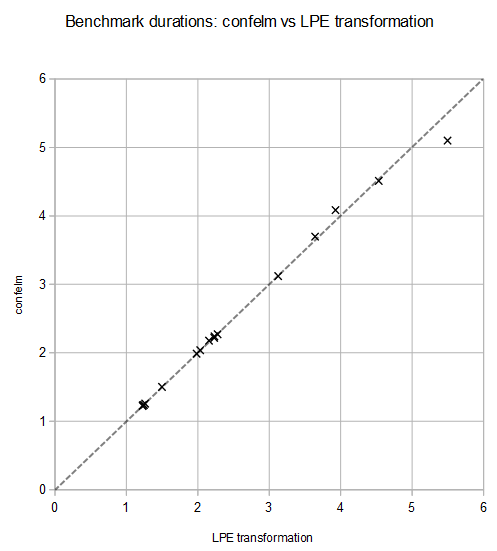
\includegraphics[width=0.7\linewidth]{charts/confelm-vs-lpe-only}
\caption{Benchmark results: confelm vs LPE transformation}
\label{confelm-vs-lpe-only:fig}
\end{center}
\end{figure}



%\chapter{istepelm}

\section{Introduction}

An LPE may contain \istep{} summands: summands that communicate exclusively over the \istep{} channel.
This indicates an invisible action of the LPE.

The \texttt{istepelm} command removes \istep{} summands from an LPE at the cost of additional summands.
The resulting LPE preserves the behavior of the original LPE only up to weak (branching?) bisimulation.

Removing \istep{} may make exploration of the LPE more efficient, especially when the LPE contains \istep{} loops.

\section{Implementation}

TODO I do not believe that there is a viable implementation anymore...!

\section{Example}

TODO

%\input{mcrl2}
\chapter{isdet} \label{isdet}

\section{Introduction}

The \texttt{isdet} command checks whether the specified LPE is deterministic.
The command may yield false negatives.

\section{Formal background}

\subsection{Summand determinism}

Consider two summands, $s_\alpha$ and $s_\beta$, and reference their elements conform \ref{summandelements}.

Summands $s_\alpha$ and $s_\beta$ are said to be \emph{deterministic} if one of these conditions holds:

\begin{itemize}
\item $s_\alpha$ and $s_\beta$ are the same summand; that is, $s_\alpha = s_\beta$.

\item $s_\alpha$ and $s_\beta$ communicate over different channels:
\begin{align*}
C_\alpha \neq C_\beta \land (C_\alpha \in \{\istep{}, \cistep{}\} \not\leftrightarrow C_\beta \in \{\istep{}, \cistep{}\})
\end{align*}

\item $s_\alpha$ and $s_\beta$ communicate with different numbers of communication variables; that is, $m_\alpha \neq m_\beta$.

\item $s_\alpha$ and $s_\beta$ are never simultaneously enabled, or $s_\alpha$ and $s_\beta$ always lead to the same next state.
In order to determine this, check if
\begin{align*}
g_\alpha[X_\beta] \land g_\beta \rightarrow \bigwedge\limits_{j=1}^{k} v_\alpha(p_j)[X_\beta] = v_\beta(p_j)
\end{align*}

is a tautology, where $X_\beta$ is defined as
\begin{align*}
X_{\beta} &= [x_\alpha(j) \rightarrow x_\beta(j) \;|\; 1 \leq j \leq \text{min}(m_\alpha, m_\beta)]
\end{align*}
\end{itemize}

Note that this approach is \emph{not} guaranteed to correctly recognize that two summands are deterministic (false negatives are tolerated)!

\section{Algorithm}

The algorithm invoked by the \texttt{isdet} command checks for all pairs of different summands whether the first summand is deterministic with the second summand (see the previous section).
The algorithm yields \textbf{true} if and only if this is the case for all summand pairs.

\section{Example}

Consider the following LPE:

\begin{lstlisting}
//Process definition:
PROCDEF example[A :: Int](x, y :: Int)
  = A ? i [[x==0 /\ i>=0 /\ i<=5]] >-> example[A](1, 0)
  + A ? i [[y==0 /\ i>=5 /\ i<=9]] >-> example[A](0, 1)
  ;

//Initialization:
example[A](0, 1);
\end{lstlisting}

Consider the two summands, calling the first $s_1$ and the second $s_2$.

The first three conditions for detecting determinism are false.

For the fourth condition, the antecedent is
\begin{align*}
g_1[X_2] \land g_2 &\Leftrightarrow (\texttt{x} = 0 \land \texttt{i} \geq 0 \land \texttt{i} \leq 5)[\texttt{i} \rightarrow \texttt{i}] \land (\texttt{y} = 0 \land \texttt{i} \geq 5 \land \texttt{i} \leq 9) \\
&\Leftrightarrow \texttt{x} = 0 \land \texttt{y} = 0 \land \texttt{i} = 5
\end{align*}

Given the antecedent, the conclusion must hold.
This is not the case:
\begin{align*}
v_1(\texttt{x})[X_2] = 1[\texttt{i} \rightarrow \texttt{i}] = 1 \neq 0 = v_2(\texttt{x}) \\
v_1(\texttt{y})[X_2] = 0[\texttt{i} \rightarrow \texttt{i}] = 0 \neq 1 = v_2(\texttt{y}) \\
\end{align*}

$s_1$ is therefore \emph{not} deterministic with $s_2$.

Changing the LPE to

\begin{lstlisting}
//Process definition:
PROCDEF example[A :: Int](x, y :: Int)
  = A ? i [[x==0 /\ i>=0 /\ i<=4]] >-> example[A](1, 0)
  + A ? i [[y==0 /\ i>=5 /\ i<=9]] >-> example[A](0, 1)
  ;

//Initialization:
example[A](0, 1);
\end{lstlisting}

will result in an antecedent that is false; therefore, $s_1$ is deterministic with $s_2$.


\chapter{det}

\section{Introduction}

Non-determinism in an LPE can have a strong impact on the performance of exploring its state space.
Preferably, an LPE should therefore be completely deterministic.
Unfortunately, there are no determinization methods known for symbolic models such as LPEs.

The \texttt{det} command described in this section is only a naive attempt at LPE determinization: it looks for two summands that are non-deterministic (see \ref{isdet}), and then rewrites the LPE so that these summands have become deterministic.
This may mean that the entire LPE has become deterministic, but more typically the non-determinism will have moved to a different part of the LPE.

The \texttt{det} command is intended to be repeated in the hope that non-determinism eventually disappears from the LPE.
It is definitely possible that this may never happen!
It is also likely that the LPE will grow very large; it is therefore advised to symbolically reduce the LPE using other LPE operations after each application of \texttt{det}.

\section{Algorithm}

Let the input LPE model be $M$ and the underlying LPE be $P$, and let two summands of $P$, $s_\alpha$ and $s_\beta$, be non-deterministic (see \ref{isdet}).
Elements of $s_\alpha$ and $s_\beta$ are referenced conform \ref{summandelements}.
Define
\begin{align*}
C_{\alpha,\beta} &= C_\alpha = C_\beta \\
m_{\alpha,\beta} &= m_\alpha = m_\beta \\
X_\alpha &= [ x_\beta(j) \rightarrow x_\alpha(j) \;|\; 1 \leq j \leq m_{\alpha,\beta} ] \\
X_\beta &= [ x_\alpha(j) \rightarrow x_\beta(j) \;|\; 1 \leq j \leq m_{\alpha,\beta} ]
\end{align*}

and let $y(j)$ be a bijective function that yields fresh variables for $1 \leq j \leq m_{\alpha,\beta}$.

The \texttt{det} algorithm follows these steps:

\begin{enumerate}
\item Create a new LPE $P'$ with the same parameters as $P$, but without any summands.
Create a new LPE model $M'$ that has the same definition as $M$, except that its references to $P$ have been replaced by references to $P'$.

\item Add a new, fresh parameter $f$ of type \texttt{Bool} to $P'$.
Where $M'$ instantiates $P'$, initialize $f$ with $\textbf{false}$.

\item Add a new, fresh parameter $Y$ to $P'$, which is a substitution from variables to values -- in practice, this is implemented with multiple parameters and/or a data hierarchy.
Where $M'$ instantiates $P'$, initialize $Y$ with $[]$.

\item Add to $P'$ each summand $s_i, i \neq \alpha, \beta$ of $P$ after changing the guard of $s_i$ from $g_i$ to $\neg f \land g_i$.

\item Add to $P'$ two new summands ${s_\alpha}'$ and ${s_\beta}'$ that are defined as
\begin{align*}
{s_\alpha}' = C_{\alpha,\beta} \; \texttt{?} \; x_\alpha(1) \; &\cdots{} \; \texttt{?} \; x_\alpha(m_{\alpha,\beta}) \; [[\neg f \land g_\alpha \land \neg g_\beta[X_\alpha]]] \\
&\texttt{>->} \; P(v_\alpha(p_1), \cdots{}, v_\alpha(p_k), \textbf{false}, []) \\
{s_\beta}' = C_{\alpha,\beta} \; \texttt{?} \; x_\beta(1) \; &\cdots{} \; \texttt{?} \; x_\beta(m_{\alpha,\beta}) \; [[\neg f \land \neg g_\alpha[X_\beta] \land g_\beta]] \\
&\texttt{>->} \; P(v_\beta(p_1), \cdots{}, v_\beta(p_k), \textbf{false}, [])
\end{align*}

\item Add to $P'$ a new summand ${s_{\alpha,\beta}}'$ that is defined as
\begin{align*}
{s_{\alpha,\beta}}' &= C_{\alpha,\beta} \; \texttt{?} \; x_\alpha(1) \; \cdots{} \; \texttt{?} \; x_\alpha(m_{\alpha,\beta}) \; [[\neg f \land g_\alpha \land g_\beta[X_\alpha]]] \\
&\texttt{>->} \; P(p_1, \cdots{}, p_k, \textbf{true}, [y(1) \rightarrow x_\alpha(1), \cdots{}, y(m_{\alpha,\beta}) \rightarrow x_\alpha(m_{\alpha,\beta})])
\end{align*}

\item For $i \in \{\alpha, \beta\}$ and for each possible successor $s_\gamma$ of $s_i$ (see \ref{possiblesuccessors}) in $P$, add to $P'$ a new summand ${s_\gamma}'$ that is defined as
\begin{align*}
{s_\gamma}' = C_\gamma \; \texttt{?} \; x_\gamma(1) \; &\cdots{} \; \texttt{?} \; x_\gamma(m_\gamma) \; [[f \land g_\gamma[Y_i]]] \\
&\texttt{>->} \; P(v_\gamma(p_1)[Y_i], \cdots{}, v_\gamma(p_k)[Y_i], \textbf{false}, [])
\end{align*}

where
\begin{align*}
Y_i &= [ p_j \rightarrow v_i(p_j)[\overline{Y_i}][Y] \;|\; 1 \leq j \leq k ] \\
\overline{Y_i} &= [x_i(1) \rightarrow y(1), \cdots{}, x_i(m_{\alpha,\beta}) \rightarrow y(m_{\alpha,\beta})]
\end{align*}

\end{enumerate}

Intuitively, the specific non-deterministic behavior of summands $s_\alpha$ and $s_\beta$ is preserved by summand ${s_{\alpha,\beta}}'$, while summands ${s_\alpha}'$ and ${s_\beta}'$ cover the deterministic behavior.
The $f$ parameter indicates that the process has just taken the non-deterministic action of ${s_\gamma}'$, and the $Y$ parameter contains the exact communication values of that action.

If $f$ is \textbf{false}, $P'$ has the same behavior as $P$ because the summands that are created in steps 4 to 6.
If $f$ is \textbf{true}, $P'$ also has the same behavior as $P$, but in such a way that the changes of summands $s_\alpha$ and $s_\beta$ are applied retroactively.

\section{Example}

Consider the following LPE:

\begin{lstlisting}
//Process definition:
PROCDEF example[A :: Int, B, C](x, y :: Int)
  = A ? i [[x==0 /\ i>=0 /\ i<=5]] >-> example[A, B, C](1, i+1)
  + A ? i [[x==0 /\ i>=5 /\ i<=9]] >-> example[A, B, C](1, i-1)
  + B [[x==1 /\ y<=4]] >-> example[A, B, C](0, 0)
  + C [[x==1 /\ y>=5]] >-> example[A, B, C](0, 0)
  ;

//Initialization:
example[A, B, C](0, 0);
\end{lstlisting}

Consider the first two summands, calling the first $s_1$ and the second $s_2$.
These summands are non-deterministic.

Applying the steps of the \texttt{det} algorithm causes the following changes:

\begin{enumerate}
\item A new LPE model $M'$ and new LPE $P'$ are created.
\item $P'$ is extended with a new parameter $\texttt{f}$.
\item $P'$ is extended with a new parameter $\texttt{z}$ (a singleton substitution).
\item The \texttt{B} and \texttt{C} summands of the input LPE are added with modified guards.
\item Based on $s_1$ and $s_2$, summands ${s_1}'$ and ${s_2}'$ are created and added.
\item Based on $s_1$ and $s_2$, summand ${s_{1, 2}}'$ is created and added.
\item The possible successors of $s_1$ and $s_2$ are the \texttt{B} and \texttt{C} summands of the input LPE, which results in 2 new \texttt{B} summands and 2 new \texttt{C} summands.
\end{enumerate}

This gives the following output LPE:

\begin{lstlisting}
PROCDEF example'[A :: Int, B, C](x, y :: Int, f: Bool, z: Int)
  = B [[not(f) /\ x==1 /\ y<=4]]
          >-> example'[A, B, C](0, 0, false, 0)
  + C [[not(f) /\ x==1 /\ y>=5]]
          >-> example'[A, B, C](0, 0, false, 0)
  + A ? i [[not(f) /\ x==0 /\ i>=0 /\ i<5]]
          >-> example'[A, B, C](1, i, false, 0)
  + A ? i [[not(f) /\ x==0 /\ i>5 /\ i<=9]]
          >-> example'[A, B, C](1, i, false, 0)
  + A ? i [[not(f) /\ x==0 /\ i==5]]
          >-> example'[A, B, C](x, y, true, i)
  + B [[f /\ z+1<=4]] >-> example[A, B, C](0, 0, false, 0)
  + B [[f /\ z-1<=4]] >-> example[A, B, C](0, 0, false, 0)
  + C [[f /\ z+1>=5]] >-> example[A, B, C](0, 0, false, 0)
  + C [[f /\ z-1>=5]] >-> example[A, B, C](0, 0, false, 0)
  ;

//Initialization:
example'[A, B, C](0, 0, false, 0);
\end{lstlisting}

The non-determinism has moved to the \texttt{B} and \texttt{C} summands at the bottom.
A subsequent application of the \texttt{clean} command removes one of the \texttt{B} summands at the bottom (because
\begin{align*}
z+1<=4 \rightarrow z-1<=4
\end{align*}

the second \texttt{B} summand \emph{contains} the first) and one of the \texttt{C} summands at the bottom (because
\begin{align*}
z-1>=5 \rightarrow z+1>=5
\end{align*}

the first \texttt{C} summand \emph{contains} the second).
Afterwards, the LPE is completely deterministic.





\chapter{uguard}

\section{Introduction}

\txs{} checks whether or not there is \emph{input-output-conformance} of an implementation with the \emph{underspecified} traces of its specification (u-ioco, see \cite{volpato2013towards}).
In this context, the specification has only to be u-ioco with itself, and it can therefore potentially be rewritten more aggressively than when a models must preserve a stronger equivalence relation.

Unfortunately, there is no information about the traces of a model that can be extracted directly from that model while it is in LPE form.
The \texttt{uguard} command is an attempt to symbolically detect a specific, relatively simple pattern with actions that do not follow the u-ioco definition.
Upon detection, the command adds guards to the LPE to exclude the underspecified actions from the model (hence its name).

\section{Formal background}

\subsection{Summand implication}

Consider two summands, $s_\alpha$ and $s_\beta$, and reference their elements conform \ref{summandelements}.

Summand $s_\alpha$ is said to \emph{imply} $s_\beta$ if these two conditions hold:

\begin{itemize}
\item $s_\alpha$ and $s_\beta$ must communicate over the exact same channel with exactly as many channel variables; that is, $C_\alpha = C_\beta \land m_\alpha = m_\beta$.

\item Define the mapping
\begin{align*}
X_\beta = [x_\alpha(j) \rightarrow x_\beta(j) \;|\; 1 \leq j \leq \text{min}(m_1, m_2)]
\end{align*}

The following condition must be a tautology:
\begin{align*}
g_\alpha[X_\beta] \rightarrow g_\beta
\end{align*}
\end{itemize}

\subsection{Possible input-successors}

Consider a summand pair $(s_\alpha, s_\beta)$, referencing the elements of $s_\alpha$ and $s_\beta$ conform \ref{summandelements}.
Summand $s_\beta$ is said to be a \emph{possible input-successor} of $s_\alpha$ if $C_\beta$ is an input channel and if the following expression is satisfiable:
\begin{align*}
g_\alpha \land {g_\beta}[v \rightarrow q(v) \;|\; v \in \varsof{g_\beta} \setminus P][p \rightarrow v_\alpha(p) \;|\; p \in P]
\end{align*}

where $q(v)$ is a bijective function that relates variable $v$ to a fresh variable.

\subsection{Definite input-successors}

Consider a summand pair $(s_\alpha, s_\beta)$, referencing the elements of $s_\alpha$ and $s_\beta$ conform \ref{summandelements}.
Summand $s_\beta$ is said to be a \emph{definite input-successor} of $s_\alpha$ if $C_\beta$ is an input channel and if the following expression is a tautology:
\begin{align*}
g_\alpha \rightarrow {g_\beta}[v \mapsto q(v) \;|\; v \in \varsof{g_\beta} \setminus P][p \mapsto v_\alpha(p) \;|\; p \in P]
\end{align*}

where $q(v)$ is a bijective function that relates variable $v$ to a fresh variable.

\section{Algorithm}

Let the input LPE model be $M$ and the underlying LPE be $P$.
The \texttt{uguard} algorithm follows these steps for all summand pairs $(s_\alpha, s_\beta)$ such that $s_\alpha$ implies $s_\beta$:

\begin{enumerate}
\item Compute $\Delta = (D_\beta \setminus P_\alpha) \cup (D_\alpha \setminus P_\beta)$ where
\begin{itemize}
\item $P_\alpha$ is the set of all possible input-successors of $s_\alpha$;
\item $P_\beta$ is the set of all possible input-successors of $s_\beta$;
\item $D_\alpha$ is the set of all definite input-successors of $s_\alpha$; and
\item $D_\beta$ is the set of all definite input-successors of $s_\beta$.
\end{itemize}

If $\Delta = \emptyset{}$, the \texttt{uguard} algorithm does not make any changes and stops.
Otherwise, it continues.

\item Create a new LPE $P'$ with the same parameters as $P$, but without any summands.
Create a new LPE model $M'$ that has the same definition as $M$, except that its references to $P$ have been replaced by references to $P'$.

\item Add a new, fresh parameter $f$ of type \texttt{Bool} to $P'$.
Where $M'$ instantiates $P'$, initialize $f$ with $\textbf{true}$.

\item For each summand $s_i$ of $P$ -- referencing its elements conform \ref{summandelements} -- add to $P'$ a new summand ${s_i}'$ that is defined as
\begin{align*}
{s_i}' = C_i \; \texttt{?} \; x_i(1) \; &\cdots{} \; \texttt{?} \; x_i(m_i) \; [[\Gamma(s_i) \land g_i]] \\
&\texttt{>->} \; P(v_i(p_1), \cdots{}, v_i(p_k), \Upsilon(s_i))
\end{align*}

where
\begin{align*}
\Gamma(s) = \begin{cases}
f \text{ if } s \in \Delta \\
\textbf{true} \text{ if } s \notin \Delta
\end{cases}
\end{align*}

and
\begin{align*}
\Upsilon(s) = \begin{cases}
\textbf{true} \text{ if } s \neq s_\alpha \land s \neq s_\beta \\
\textbf{false} \text{ if } s = s_\alpha \lor s = s_\beta
\end{cases}
\end{align*}
\end{enumerate}

Intuitively, the algorithm first detects that certain summands are underspecified: they are enabled after a certain action if that action is performed by summand $s_\alpha$, but they are not enabled after that action is performed by summand $s_\beta$.
The algorithm therefore makes it so that the underspecified summands are always disabled after $s_\alpha$ or $s_\beta$ (preserving equivalence up to u-ioco).


%\chapter{Results TODO}

TODO



\bibliographystyle{plainnat}
\bibliography{biblio}

\end{document}
